% Template for PLoS
% Version 3.5 March 2018
%
% % % % % % % % % % % % % % % % % % % % % %
%
% -- IMPORTANT NOTE
%
% This template contains comments intended
% to minimize problems and delays during our production
% process. Please follow the template instructions
% whenever possible.
%
% % % % % % % % % % % % % % % % % % % % % % %
%
% Once your paper is accepted for publication,
% PLEASE REMOVE ALL TRACKED CHANGES in this file
% and leave only the final text of your manuscript.
% PLOS recommends the use of latexdiff to track changes during review, as this will help to maintain a clean tex file.
% Visit https://www.ctan.org/pkg/latexdiff?lang=en for info or contact us at latex@plos.org.
%
%
% There are no restrictions on package use within the LaTeX files except that
% no packages listed in the template may be deleted.
%
% Please do not include colors or graphics in the text.
%
% The manuscript LaTeX source should be contained within a single file (do not use \input, \externaldocument, or similar commands).
%
% % % % % % % % % % % % % % % % % % % % % % %
%
% -- FIGURES AND TABLES
%
% Please include tables/figure captions directly after the paragraph where they are first cited in the text.
%
% DO NOT INCLUDE GRAPHICS IN YOUR MANUSCRIPT
% - Figures should be uploaded separately from your manuscript file.
% - Figures generated using LaTeX should be extracted and removed from the PDF before submission.
% - Figures containing multiple panels/subfigures must be combined into one image file before submission.
% For figure citations, please use "Fig" instead of "Figure".
% See http://journals.plos.org/plosone/s/figures for PLOS figure guidelines.
%
% Tables should be cell-based and may not contain:
% - spacing/line breaks within cells to alter layout or alignment
% - do not nest tabular environments (no tabular environments within tabular environments)
% - no graphics or colored text (cell background color/shading OK)
% See http://journals.plos.org/plosone/s/tables for table guidelines.
%
% For tables that exceed the width of the text column, use the adjustwidth environment as illustrated in the example table in text below.
%
% % % % % % % % % % % % % % % % % % % % % % % %
%
% -- EQUATIONS, MATH SYMBOLS, SUBSCRIPTS, AND SUPERSCRIPTS
%
% IMPORTANT
% Below are a few tips to help format your equations and other special characters according to our specifications. For more tips to help reduce the possibility of formatting errors during conversion, please see our LaTeX guidelines at http://journals.plos.org/plosone/s/latex
%
% For inline equations, please be sure to include all portions of an equation in the math environment.
%
% Do not include text that is not math in the math environment.
%
% Please add line breaks to long display equations when possible in order to fit size of the column.
%
% For inline equations, please do not include punctuation (commas, etc) within the math environment unless this is part of the equation.
%
% When adding superscript or subscripts outside of brackets/braces, please group using {}.
%
% Do not use \cal for caligraphic font.  Instead, use \mathcal{}
%
% % % % % % % % % % % % % % % % % % % % % % % %
%
% Please contact latex@plos.org with any questions.
%
% % % % % % % % % % % % % % % % % % % % % % % %

\documentclass[10pt,letterpaper]{article}
\usepackage[top=0.85in,left=2.75in,footskip=0.75in]{geometry}

% amsmath and amssymb packages, useful for mathematical formulas and symbols
\usepackage{amsmath,amssymb}

% Use adjustwidth environment to exceed column width (see example table in text)
\usepackage{changepage}

% Use Unicode characters when possible
\usepackage[utf8x]{inputenc}

% textcomp package and marvosym package for additional characters
\usepackage{textcomp,marvosym}

% cite package, to clean up citations in the main text. Do not remove.
% \usepackage{cite}

% Use nameref to cite supporting information files (see Supporting Information section for more info)
\usepackage{nameref,hyperref}

% line numbers
\usepackage[right]{lineno}

% ligatures disabled
\usepackage{microtype}
\DisableLigatures[f]{encoding = *, family = * }

% color can be used to apply background shading to table cells only
\usepackage[table]{xcolor}

% array package and thick rules for tables
\usepackage{array}

% create "+" rule type for thick vertical lines
\newcolumntype{+}{!{\vrule width 2pt}}

% create \thickcline for thick horizontal lines of variable length
\newlength\savedwidth
\newcommand\thickcline[1]{%
  \noalign{\global\savedwidth\arrayrulewidth\global\arrayrulewidth 2pt}%
  \cline{#1}%
  \noalign{\vskip\arrayrulewidth}%
  \noalign{\global\arrayrulewidth\savedwidth}%
}

% \thickhline command for thick horizontal lines that span the table
\newcommand\thickhline{\noalign{\global\savedwidth\arrayrulewidth\global\arrayrulewidth 2pt}%
\hline
\noalign{\global\arrayrulewidth\savedwidth}}


% Remove comment for double spacing
%\usepackage{setspace}
%\doublespacing

% Text layout
\raggedright
\setlength{\parindent}{0.5cm}
\textwidth 5.25in
\textheight 8.75in

% Bold the 'Figure #' in the caption and separate it from the title/caption with a period
% Captions will be left justified
\usepackage[aboveskip=1pt,labelfont=bf,labelsep=period,justification=raggedright,singlelinecheck=off]{caption}
\renewcommand{\figurename}{Fig}

% Use the PLoS provided BiBTeX style
% \bibliographystyle{plos2015}

% Remove brackets from numbering in List of References
\makeatletter
\renewcommand{\@biblabel}[1]{\quad#1.}
\makeatother



% Header and Footer with logo
\usepackage{lastpage,fancyhdr,graphicx}
\usepackage{epstopdf}
%\pagestyle{myheadings}
\pagestyle{fancy}
\fancyhf{}
%\setlength{\headheight}{27.023pt}
%\lhead{
\includegraphics[width=2.0in]{PLOS-submission.eps}}
\rfoot{\thepage/\pageref{LastPage}}
\renewcommand{\headrulewidth}{0pt}
\renewcommand{\footrule}{\hrule height 2pt \vspace{2mm}}
\fancyheadoffset[L]{2.25in}
\fancyfootoffset[L]{2.25in}
\lfoot{\today}

%% Include all macros below

\newcommand{\lorem}{{\bf LOREM}}
\newcommand{\ipsum}{{\bf IPSUM}}



\usepackage{rotating, graphicx, dcolumn, booktabs, caption, xcolor}
\usepackage{booktabs}
\usepackage{longtable}
\usepackage{array}
\usepackage{multirow}
\usepackage{wrapfig}
\usepackage{float}
\usepackage{colortbl}
\usepackage{pdflscape}
\usepackage{tabu}
\usepackage{threeparttable}
\usepackage{threeparttablex}
\usepackage[normalem]{ulem}
\usepackage{makecell}
\usepackage{xcolor}



\usepackage{forarray}
\usepackage{xstring}
\newcommand{\getIndex}[2]{
  \ForEach{,}{\IfEq{#1}{\thislevelitem}{\number\thislevelcount\ExitForEach}{}}{#2}
}

\setcounter{secnumdepth}{0}

\newcommand{\getAff}[1]{
  \getIndex{#1}{University of Bristol and The Alan Turing Institute,Tufts University}
}

\providecommand{\tightlist}{%
  \setlength{\itemsep}{0pt}\setlength{\parskip}{0pt}}

\begin{document}
\vspace*{0.2in}

% Title must be 250 characters or less.
\begin{flushleft}
{\Large
\textbf\newline{Ubiquitous Digital Technologies and Spatial Structure; an update} % Please use "sentence case" for title and headings (capitalize only the first word in a title (or heading), the first word in a subtitle (or subheading), and any proper nouns).
}
\newline
% Insert author names, affiliations and corresponding author email (do not include titles, positions, or degrees).
\\
Emmanouil Tranos\textsuperscript{\getAff{University of Bristol and The Alan Turing Institute}}\textsuperscript{*},
Yannis M. Ioannides\textsuperscript{\getAff{Tufts University}}\\
\bigskip
\textbf{\getAff{University of Bristol and The Alan Turing Institute}}University of Bristol, School of Geographical Sciences, Bristol, UK; The
Alan Turing Institute, London, UK\\
\textbf{\getAff{Tufts University}}Tufts University, Department of Economics, Medford, MA, USA\\
\bigskip
* Corresponding author: e.tranos@bristol.ac.uk\\
\end{flushleft}
% Please keep the abstract below 300 words
\section*{Abstract}
This paper examines the impact of widespread adoption of information and
communication technologies (ICT) on urban structure worldwide. Has it
offset agglomeration benefits and led to more dispersed spatial
structures, or has it strengthened urban externalities and thus resulted
in more concentrated spatial structures? Theoretical and empirical
studies on this question have produced contradictory findings. The
present study recognizes that assumptions made earlier about the
evolution of technological capabilities do not necessarily hold today.
As cutting-edge digital technologies have matured considerably, a fresh
look at this question is called for.

The paper addresses this issue by means of several data sets using
instrumental variable methods. One is the UN data on Urban Settlements
with more than \(300,000\) inhabitants. Estimation methods with these
data show that increased adoption of ICT has resulted in national urban
systems that are less uniform in terms of city sizes and are
characterized by higher population concentrations in larger cities, when
concentration is proxied the Pareto (Zipf) coefficient for national city
size distributions. Two, is disaggregated data for the urban systems of
the US, defined as Micropolitan and Metropolitan Areas, and for the UK,
defined as Built-up Areas in England and Wales, respectively. These data
allow for the impacts to be studied for cities smaller than those
included in the cross-country data. Increased internet usage improved a
city's ranking in the US urban system. Similarly, increased download
speed improves a built-up area's ranking in England and Wales.

% Please keep the Author Summary between 150 and 200 words
% Use first person. PLOS ONE authors please skip this step.
% Author Summary not valid for PLOS ONE submissions.
\section*{Author summary}
TO ADD

\linenumbers

% Use "Eq" instead of "Equation" for equation citations.
\hypertarget{sec:1}{%
\section{Introduction}\label{sec:1}}

Geographers, planners and urban economists spent effort in exploring the
spatial footprint of the internet even at its early stages. They
theorized about the spatial impacts that rapid internet penetration
might generate on individual cities and the national spatial structure.
The outcome of various such efforts was rather conjectural and even
fanciful and not data-based. Cases in point are celebrations of the
emergence of telecottages {[}1{]}, the rise of a borderless world
{[}2{]}, the death of cities {[}3,4{]}, and, more generally, the end of
geography {[}5{]}, the death of distance {[}6{]} and the emergence of a
new flat world {[}7{]}. Today, \(25\) years after the commercialization
of the internet {[}8{]}, we know that the above narratives overstated
the potential of the internet and other digital communication
technologies to supplement face-to-face interactions, diminish the cost
of distance and, indeed weaken agglomeration economies. The high and
steadily increasing urbanization rates {[}9{]} falsify such predictions.

The adoption rate and the pervasiveness of new internet-based
information and communication technologies, ICT for short, such as
online social media and mobile-telephony hosted internet, which have
increased rapidly during the last 10-15 years in the developing world,
too, raise questions about how exactly ICT might have affected
agglomeration economies. Conflicting technology examples can be
illustrated. On the one hand, despite the broader agreement that no
digital technology can reach the content richness of face-to-face
communications, empirical research from the management field suggests
that current digital technologies can effectively facilitate the sharing
of knowledge with low to medium tacitness and even support knowledge
sharing of a high degree of tacitness {[}10{]}. On the other hand, the
very same technologies can further enhance what Storper and Venables
{[}11{]} termed as buzz, as the constant publication of our personal and
professional updates and whereabouts enabled by ICT can directly
facilitate deliberate as well as unplanned or even unintentional
face-to-face meetings {[}12{]}.

Urban economics suggests that a key source of agglomeration
externalities is proximity, which facilitates interaction and knowledge
spillovers {[}13{]}. Hence, face-to-face interactions and the implied
knowledge spillovers within cities flourish because of lower
transportation and interaction costs {[}11{]}. However, ICT have the
capacity to directly affect this process by further reducing
transportation cost {[}14{]}. In essence, the internet and digital
communications promote further learning and matching, which are at the
heart of the micro-foundations of agglomeration economies identified by
Duranton and Puga {[}15{]}. Web-based applications such as Massive Open
Online Courses decrease the need for co-location of actors in order to
participate in formal learning activities. Furthermore, online social
media such as LinkedIn can enhance the probability of matching and
indeed the quality of matches even within cities. This is why LinkedIn
has been identified as ``the largest professional matchmaker site in the
world'' {[}{[}16{]} p.~207; {[}17{]}{]}. Therefore, it is natural to ask
whether the widespread adoption of ICT could offset the benefits of
immediate physical proximity and result in more dispersed spatial
structures, or further reinforce agglomeration externalities and lead to
more concentrated spatial structures.

This paper contributes to the above discussion by presenting empirical
research on whether the internet and digital communications have
affected spatial structure, as seen via the size distribution of cities.
Contrary to most of the previous empirical studies, which are reviewed
in the next section, this paper returns first to an empirical setting
similar to that of Ioannides et al.~{[}18{]} in order to re-examine
their results by employing updated data on internet use, associated with
the enhanced technological maturity of ICT, and using a number of
different data sets. In contrast to Tranos and Ioannides {[}19{]}, which
revisits the question by seeking to replicate Ioannides et al.~{[}18{]},
but with the same but augmented data as that earlier study, the present
paper probes the significance of different levels of aggregation for the
relation between agglomeration externalities and digital communications
by employing different scales of spatial aggregation. One is a global
multi-country analysis using urban agglomeration data for many
countries; a second is a more granular analysis for the US and the UK.
For those two countries the paper brings novel data to bear on the
question. In addition, the paper also distinguishes the effects of a
broader range of ICT on spatial structure, including internet and
broadband internet as well as mobile and landline telephony adoption
rates.

Interestingly, in contrast to Tranos and Ioannides {[}19{]}, most of the
differences in the results -- from the global level analysis to the case
studies --- support a complementarity argument. Specifically, the paper
examines econometrically whether spatial structures have been affected
by the adoption rates of the different digital communication
technologies described above. The results are robust against potential
endogeneity concerns, as one might claim that the take-up of these
technologies could have been affected by spatial structures themselves.
That is, individuals living in more dispersed spatial systems might have
made greater use of such technologies in order to overcome the lower
level of agglomeration externalities. Notably, we find some evidence
that such effects are stronger in smaller urban areas. Our findings can
directly inform the urban policy agenda as they advocate in favor of
including digital strategies in policies aiming to enhance agglomeration
externalities and to improve the position of a city within its national
urban hierarchy.

The impact of ICT adoption on urban spatial structure is of such
paramount importance in understanding its impact on modern economies
that replicating a study by extending and updating its data is a
worthwhile undertaking. By the same token, it behooves us to examine its
robustness by means of alternative data sets. Unlike the data used by
Ioannides et al {[}18{]} and Tranos and Ioannides {[}19{]}, the data
employed by the current study is arguable more consistent. The structure
of the paper is as follows: \protect\hyperlink{sec2}{Section 2} provides
a brief literature review; \protect\hyperlink{sec3}{Section 3} describes
the methods and the data we use; \protect\hyperlink{sec4}{Section 4}
presents the results of the multi-country analysis;
\protect\hyperlink{sec5}{Section 5} narrows down to the two case
studies, the US and UK; and, \protect\hyperlink{sec6}{Section 6}
concludes.

\hypertarget{sec2}{%
\section{Literature review}\label{sec2}}

Gaspar and Glaeser {[}20{]} were the first to model the effect of
telecommunication improvements on the intensity of face-to-face
interactions and city size. Their results indicate that technological
improvements in telecommunications may lead to increased demand for
face-to-face interactions, which will then increase the importance of
cities. Their theoretical model allows for a complementary relation
between agglomeration externalities and advances in telecommunications.
However, their results rest on a critical assumption, namely that
face-to-face interactions are superior to any technology-mediated
interactions. Were it not for this assumption then the opposite
prediction would have followed. As indicated above and as the management
literature suggests, face-to-face interactions do not necessarily
dominate digitally mediated ones. Certain elements of knowledge sharing
can also be achieved by via online interactions {[}10,21{]}. Indeed, to
a certain extent, this argument is technology dependent. E.g., current
teleconferencing capabilities are much more advanced than the ones
available in the late 1990s. Hence, it behooves us to return empirically
to the impact on agglomeration externalities from improved
telecommunication technologies.

Kolko {[}22{]} uses internet diffusion data and identifies a clear
complementary link between internet usage and city size. Interestingly,
he identifies higher internet domain densities in remote cities which
indicates a substitution effect of the internet for longer-distance
non-electronic communications. His results are consistent for different
measures of internet diffusion (internet domain density and internet
take-up). Sinai and Waldfogel {[}23{]} approach the same question from
the consumers' point of view and find support for complementarity
between internet and cities. They study the link between market size and
locally targeted online content and find more online local content in
larger markets. However, they also obtain evidence for a substitution
effect: holding local online content constant, market size has a
negative effect on individual connectivity. Forman et al.~{[}24{]}
examines whether commercial internet adoption is higher in cities than
in rural areas. While the former would indicate a complementarity
between internet adoption and cities, the latter would reflect a
substitutability relation, according to which the internet is used as a
means to offset costs and lack of opportunities related to
peripheriality. Their results indicate that despite internet adoption by
firms with more than 100 employees being greater in smaller urban
agglomerations, the adoption of more sophisticated internet-based
applications is positively related with city size in \(2000\). Sohn,
Kim, and Hewings {[}25{]} compare how information technologies are
related to urban spatial structure for Chicago and Seoul. Although they
find a clear complementary link for Chicago, this is not the case for
Seoul, where information technologies contribute to a more dispersed
spatial pattern. Focusing on the municipalities in the province of
Barcelona, Pons-Novell and Viladecans-Marsal {[}26{]} find a
complementary link between individual internet take-up and off-line
commercial offerings, but their results cannot safely reject a
substitution effect. Craig, Hoang, and Kohlhase {[}27{]} focus on
internet take-up rates across US states during the period \(2000-2011\).
Their analysis provides suggestive evidence of a complementary role that
internet connectivity performs on urban living. Ioannides et
al.~{[}18{]} use country-level data on city size distributions to
examine the impact of fixed line telephony on urban structure
\(1980-2000\). Using a panel dataset of spatial dispersion measures,
they find robust evidence that an increase in the number of telephone
lines per capita encourages the spatial dispersion of population in that
they lead to a more concentrated distribution of city sizes. In
addition, by the end of their study period the internet has come into
use, but their results with internet usage is more speculative but do
show that it goes in the same direction.

Focusing on rural areas, Partridge et al.~{[}28{]} find no evidence that
rural distance penalties in the US have substantially changed since
\(1970s\) indicating that technological changes including the internet
and digital communications have not affected spatial structure. Also
interesting are the findings of a more recent study by Kim and Orazem
{[}29{]} on the economic effects of broadband internet in rural areas.
They identify a positive effect on new firm location decisions, with the
effect being higher in rural areas with larger population and in rural
areas adjacent to a metropolitan area. These results suggest a
complementary relation between the internet and agglomeration economies.

Moving beyond modelling the direct relationship between ICT and spatial
structure, Bekkerman and Gilpin {[}30{]} focused on the role of locally
based information resources using a dataset about the US libraries
during the period \(2000-2008\). Their results suggest that internet
access increases the demand and the value of locally accessible
information, and such complementarities are higher in larger
metropolitan areas. Anenberg and Kung {[}31{]} also identified a
complementary relation between the internet and consumption variety in
cities by focusing on food truck industry in the US.

Thus, clearly, previous research suggests that the declaration of the
``death of distance'' has proven to be premature {[}32{]}. However, the
exact impact of digital communications on spatial structure is still an
open question. As Leamer and Storper {[}33{]} indicate, the internet can
affect both centripetal and centrifugal forces. The only cross country
study {[}18{]} supports a clear substitution effect, whereas most of the
above studies have focused either on the US or on some specific cities.
Moreover, most of the above studies examined the
complementarity/substitutability question over time periods when the
internet and other digital communication technologies were still
emerging. For instance, internet penetration in the US in \(2000\),
which was the focus for quite a few of the above studies including
Ioannides et al.~{[}18{]}, was just above \(50\) percent, while in
\(2016\) it reached almost \(90\) percent {[}34{]}. At a global scale
internet penetration increased from \(7\) to \(46\) percent during the
same period {[}35{]}. In addition, although email and instant messaging
technologies were widespread in the developed world in early \(2000s\),
network externalities due to mobile internet and online social media
were nowhere close to what we are familiar with today. For instance,
Facebook users increased from \(1\) million in \(2004\) to more than
\(1.5\) billion in \(2015\) {[}36{]}. Hence, it might have been
premature for the spatial economic effects of ICT adoption to have been
materialized by the time that most of the above studies were conducted.

Most recently, Tranos and Ioannides {[}19{]} return to the setting of
Ioannides et al.~{[}18{]}, update the data employed and obtain results
that confirm their original findings. That is, the diffusion of fixed
telephony has caused more dispersed urban structures worldwide, in other
words, greater urban decentralization. Similar causal effects are
established for mobile telephony, which are novel in relation to
Ioannides et al.~{[}18{]}, who lacked such data, and for the internet,
which extends their earlier findings. The robustness of their results is
confirmed for such alternative measures of dispersion as the Gini
coefficient, the Herfindahl index, and the coefficient of variation.
This is notable because several years of additional data were used that
pertain to an era of rapid expansion of the internet and web-based
technologies, more generally.

The present paper does not address the issue that adoption of ICT may
have different effects on urban dispersion on a national scale, that is
how far are major urban areas, that is, cities, from one another, versus
dispersion within major urban areas, that is urban sprawl. Such an
inquiry would require detailed data about patterns of how urban sprawl
may hamper or promote economic interaction, given advancements in
information technology. We think that data from the Covid-19 pandemic
would likely throw light at this issue in the future, as it is clear
that not all economic activities might continue in an unencumbered
manner; see Dingel and Neiman {[}37{]}.

\hypertarget{sec3}{%
\section{Materials and Methods}\label{sec3}}

The main aim of this paper is to return to the estimation of the causal
impact of ICT adoption on the spatial dispersion of economic activities
and consequently population. It adopts an approach that is carried out
at several spatial scales and uses different data than those used by
Ioannides et al.~{[}18{]} and Tranos and Ioannides {[}19{]}.

We start with a multi-country exercise, which includes both developed
and developing countries. \protect\hyperlink{sec3.1}{Section 3.1}
discusses the methods and the different data we use and
\protect\hyperlink{sec4}{Section 4} reports the results. Because of
limitations related with multi-country urban population data (see
discussion below), we complement our analysis with two case studies for
the US and the UK urban system for which we have access to much more
granular data. \protect\hyperlink{sec3.2}{Section 3.2} discusses the
methods and \protect\hyperlink{sec5}{Section 5} reports the results.

\hypertarget{sec3.1}{%
\subsection{Multi-country analysis}\label{sec3.1}}

The multi-country identification strategy is a two-step approach
{[}18{]}. The first step of our methodology is to estimate the Pareto
exponent for a broad sample of countries over time. The Pareto exponent
is one of the most widely used measures of spatial dispersion with
numerous applications in urban economics and economic geography ({[}see
for example {[}38{]}; {[}39{]}; {[}40{]}; {[}41{]}; {[}42{]}; {[}43{]};
{[}44{]}). This an appropriate measure of dispersion because of the
extreme heterogeneity of the city size distribution and the very good
fits normally obtained with such estimations. We also replicate our
analysis using other measures of dispersion in Appendix S1. Our results
remain consistent. Skipping details pertaining of the suitability of the
approach, which may be found in Ioannides et al.~{[}18{]} and Tranos and
Ioannides {[}19{]}, we proceed with the estimation of the logarithmic
form of:

\begin{align}
ln(rank_{i}) = ln(S_0) + \zeta ln(Size_i) + e_{i}. \label{eq1}
\end{align}

This leads to an estimate of \(\zeta\), known as the Zipf coefficient,
but more appropriately the Pareto exponent, a terminology we will adhere
to for the remained of the text, even when \(\zeta\) is estimated to be
near \(1\). The term Zipf coefficient should be reserved for the special
case of \(\zeta=1\). While much of the literature focuses on the Pareto
exponent being close to \(1\), several estimations of city size
distributions lead to estimates of \(\zeta\) that are not necessarily
equal to \(1\), or even near it, in which case we refer to \(\zeta\) as
the Pareto, or power law, exponent. Given that our aim here is to
estimate \(\zeta\) for a number of countries over time as a measure of
dispersion, equation \ref{eq1} describes the rank of city \(i\) in
country \(c\) in year \(t\):

\begin{align}
ln(rank_{ict}) = ln(S_{0ct}) + \zeta_{ct} ln(Size_{ict}) + e_{ict}. \label{eq2}
\end{align}

The estimation of equation \ref{eq2} has typically been performed by
Ordinary Least Squares (OLS). Gabaix and Ioannides {[}45{]} discuss the
downward bias of estimates of equation \ref{eq2} using OLS on small
samples. Gabaix and Ibragimov {[}46{]} propose a practical remedy to
correct this bias, which we do adopt in this paper: instead of using the
\(log\) of \(rank\) of a city \(i\) in a country \(c\) in year \(t\),
they propose to use the \(log(rank-0.5)\), which has indeed been widely
adopted. Researchers working in this area must contend with definitional
differences as well as differences in availability of different kinds of
data sources. Definitions of cities differ across countries, for
political, administrative and legal reasons {[}see {[}47{]}, Ch. 8, for
issues and pitfalls associated with different definitions{]}. In
contrast to the data drawn from Thomas Brinkhoff's City Population
project {[}48{]}, which were used by Soo {[}49{]}, Ioannides et
al.~{[}18{]} and Tranos and Ioannides {[}19{]}, the multi-country
analysis in the present paper is based on the annual population data for
urban agglomerations with \(300,000\) inhabitants or more from the
Department of Economic and Social Affairs of the United Nations {[}9{]}.
Despite some criticism about the consistency of the urban agglomeration
definitions across different countries {[}50{]}, this is the only
available source for yearly, multi-country population data for urban
agglomerations {[}51--53{]}. The results based on these data are
reported and discussed in \protect\hyperlink{sec4}{Section 4}.

Table \ref{zipf} presents the estimated \(\zeta\) coefficients for the
panel of countries that the second stage of the analysis focuses on
using the UN urban agglomerations data. More detailed and interactive
visualisations can be found in Appendix S2. It becomes evident that
there is considerable variation in the estimates of \(\zeta\) across the
different countries in the sample. Because of the empirically
established heavy upper tail of data for cities and urban
agglomerations, the \(\zeta\) coefficient constitutes a convenient
measure of dispersion. The larger its absolute value, the thinner the
upper tail; equivalently, the larger is the coefficient algebraically,
the heavier the upper tail. This key observation is basis for the second
step of our methodology.

\begin{table}

\caption{\label{tab:unnamed-chunk-2}Pareto exponents\label{zipf}}
\resizebox{\linewidth}{!}{
\begin{tabular}[t]{lrrrrrrrrrrrrrrrrrrr}
\toprule
Countries & 2000 & 2001 & 2002 & 2003 & 2004 & 2005 & 2006 & 2007 & 2008 & 2009 & 2010 & 2011 & 2012 & 2013 & 2014 & 2015 & 2016 & 2017 & 2018\\
\midrule
AGO & NA & -0.94 & -0.94 & -0.94 & -0.94 & -0.94 & -0.93 & -0.93 & -0.92 & -0.92 & -0.92 & -0.91 & -0.90 & -0.90 & -0.89 & -0.90 & -0.90 & -0.91 & NA\\
ARG & -0.97 & -0.97 & -0.97 & -0.97 & -0.97 & -0.97 & -0.97 & -0.97 & -0.97 & -0.97 & -0.97 & -0.97 & -0.97 & -0.98 & -0.98 & -0.98 & -0.98 & -0.98 & NA\\
AUS & -0.82 & -0.82 & NA & NA & NA & -0.83 & -0.83 & -0.82 & -0.82 & -0.82 & -0.82 & -0.82 & -0.81 & -0.81 & -0.81 & -0.81 & -0.81 & -0.80 & NA\\
BGD & -0.65 & -0.65 & -0.66 & -0.67 & -0.67 & -0.68 & -0.69 & -0.69 & -0.70 & -0.70 & -0.71 & -0.72 & -0.72 & -0.72 & -0.73 & -0.73 & -0.73 & -0.73 & NA\\
BLR & -1.26 & -1.26 & -1.26 & NA & NA & NA & -1.24 & -1.23 & -1.23 & -1.22 & -1.22 & -1.23 & -1.23 & -1.23 & -1.23 & -1.23 & -1.23 & -1.23 & -1.23\\
\addlinespace
BRA & -0.93 & -0.93 & -0.93 & -0.93 & -0.93 & -0.93 & -0.93 & -0.93 & -0.93 & -0.93 & -0.94 & -0.94 & -0.94 & -0.94 & -0.94 & -0.94 & -0.94 & -0.93 & -0.93\\
CAN & -1.06 & -1.05 & -1.05 & -1.05 & -1.05 & -1.04 & -1.04 & -1.04 & -1.04 & -1.03 & -1.03 & -1.03 & -1.03 & -1.02 & -1.02 & -1.02 & -1.02 & NA & NA\\
CHL & -0.73 & -0.73 & -0.73 & -0.74 & -0.74 & -0.75 & -0.75 & -0.76 & -0.76 & -0.76 & -0.77 & -0.77 & -0.77 & -0.78 & -0.78 & -0.78 & -0.78 & -0.79 & NA\\
CHN & -1.15 & -1.16 & -1.16 & -1.17 & -1.17 & -1.18 & -1.18 & -1.18 & -1.19 & -1.19 & -1.19 & -1.19 & -1.19 & -1.20 & -1.20 & -1.20 & -1.20 & -1.21 & NA\\
CMR & -0.76 & -0.76 & -0.76 & -0.76 & -0.76 & -0.77 & -0.77 & -0.77 & -0.77 & -0.76 & -0.76 & -0.76 & -0.76 & -0.76 & -0.77 & -0.77 & -0.77 & -0.77 & NA\\
\addlinespace
COD & -0.94 & -0.94 & -0.95 & -0.95 & -0.96 & -0.96 & -0.97 & -0.97 & -0.98 & -0.98 & -0.99 & -0.99 & -0.99 & -0.99 & -0.99 & -0.99 & -1.00 & -1.00 & NA\\
COL & -0.98 & -0.98 & -0.98 & -0.98 & -0.98 & -0.98 & -0.98 & -0.98 & -0.98 & -0.98 & -0.98 & -0.98 & -0.98 & -0.98 & -0.98 & -0.98 & -0.98 & -0.98 & -0.98\\
DEU & -1.53 & -1.53 & -1.53 & -1.53 & -1.53 & -1.52 & -1.52 & -1.52 & -1.51 & -1.51 & -1.51 & -1.51 & -1.50 & -1.50 & -1.50 & -1.50 & -1.50 & -1.50 & -1.50\\
DZA & -1.10 & -1.11 & -1.12 & -1.13 & -1.14 & -1.15 & -1.15 & -1.16 & -1.16 & -1.17 & -1.18 & -1.18 & -1.18 & -1.19 & -1.19 & -1.19 & -1.19 & -1.20 & -1.21\\
EGY & -0.73 & -0.73 & -0.73 & -0.73 & -0.73 & -0.73 & -0.73 & -0.73 & -0.72 & -0.72 & -0.72 & -0.72 & -0.72 & -0.72 & -0.72 & -0.72 & -0.72 & -0.71 & -0.71\\
\addlinespace
ESP & -0.94 & -0.94 & -0.93 & -0.93 & -0.93 & -0.93 & -0.93 & -0.92 & -0.92 & -0.92 & -0.92 & -0.92 & -0.91 & -0.91 & -0.91 & -0.91 & -0.91 & -0.90 & -0.90\\
FRA & -1.15 & -1.15 & -1.15 & -1.15 & -1.14 & -1.14 & -1.14 & -1.14 & -1.14 & -1.14 & -1.14 & -1.14 & -1.14 & -1.14 & -1.13 & -1.13 & -1.13 & -1.13 & -1.13\\
GBR & -1.19 & -1.19 & -1.19 & -1.19 & -1.19 & -1.19 & -1.19 & -1.19 & -1.18 & -1.18 & -1.18 & -1.18 & -1.18 & -1.17 & -1.17 & -1.17 & -1.17 & -1.17 & -1.16\\
IDN & -1.11 & -1.11 & -1.12 & -1.12 & -1.12 & -1.13 & -1.13 & -1.13 & -1.13 & -1.13 & -1.13 & -1.13 & -1.13 & -1.13 & -1.13 & -1.13 & -1.12 & -1.12 & -1.12\\
IND & -1.05 & -1.06 & -1.06 & -1.06 & -1.07 & -1.07 & -1.08 & -1.08 & -1.08 & -1.09 & -1.09 & -1.09 & -1.09 & -1.09 & -1.09 & -1.09 & -1.09 & -1.09 & NA\\
\addlinespace
IRN & -1.03 & -1.05 & -1.07 & -1.09 & -1.11 & -1.13 & -1.14 & -1.15 & -1.16 & -1.16 & -1.17 & -1.17 & -1.18 & -1.18 & -1.18 & -1.19 & -1.19 & -1.19 & NA\\
IRQ & NA & -1.06 & -1.07 & -1.07 & -1.08 & -1.07 & -1.07 & -1.07 & -1.05 & -1.03 & -1.06 & -1.10 & -1.14 & -1.17 & -1.20 & -1.24 & -1.23 & -1.23 & -1.23\\
ITA & -1.38 & -1.39 & -1.39 & -1.39 & -1.40 & -1.40 & -1.40 & -1.41 & -1.41 & -1.41 & -1.42 & -1.42 & -1.42 & -1.43 & -1.43 & -1.43 & -1.44 & -1.44 & -1.44\\
JOR & -0.94 & -0.97 & -1.00 & -1.04 & -1.07 & -1.09 & -1.11 & -1.12 & -1.13 & -1.15 & -1.16 & -1.17 & -1.19 & -1.20 & -1.22 & -1.23 & -1.25 & -1.26 & NA\\
JPN & -0.77 & -0.77 & -0.76 & -0.76 & -0.76 & -0.76 & -0.76 & -0.75 & -0.75 & -0.75 & -0.75 & -0.75 & -0.75 & -0.75 & -0.75 & -0.75 & -0.75 & -0.75 & -0.74\\
\addlinespace
KAZ & -1.93 & -1.91 & -1.88 & -1.85 & -1.83 & -1.82 & -1.81 & -1.79 & -1.78 & -1.76 & -1.72 & -1.68 & -1.63 & -1.59 & -1.55 & -1.51 & -1.47 & -1.43 & -1.39\\
KEN & -0.75 & -0.76 & -0.77 & -0.78 & -0.79 & -0.80 & -0.80 & -0.81 & -0.81 & -0.82 & -0.82 & -0.81 & -0.81 & -0.81 & -0.81 & -0.81 & -0.81 & -0.81 & NA\\
KOR & -1.04 & -1.05 & -1.06 & -1.08 & -1.09 & -1.10 & -1.10 & -1.11 & -1.11 & -1.11 & -1.12 & -1.12 & -1.12 & -1.12 & -1.12 & -1.13 & -1.13 & -1.13 & -1.13\\
MAR & -1.23 & -1.23 & -1.23 & -1.23 & -1.23 & -1.23 & -1.23 & -1.23 & -1.24 & -1.24 & -1.24 & -1.24 & -1.24 & -1.24 & -1.24 & -1.24 & -1.24 & -1.24 & -1.24\\
MEX & -1.17 & -1.18 & -1.18 & -1.18 & -1.18 & -1.18 & -1.18 & -1.18 & -1.18 & -1.18 & -1.19 & -1.19 & -1.19 & -1.19 & -1.19 & -1.19 & -1.19 & -1.19 & -1.19\\
\addlinespace
MOZ & -1.15 & -1.16 & -1.17 & -1.18 & -1.18 & -1.19 & -1.20 & -1.21 & -1.23 & -1.24 & -1.26 & -1.26 & -1.27 & -1.28 & -1.31 & -1.34 & -1.36 & -1.38 & NA\\
MYS & -1.04 & -1.03 & -1.03 & -1.03 & -1.03 & -1.02 & -1.02 & -1.02 & -1.01 & -1.01 & -1.01 & -1.00 & -1.00 & -1.00 & -0.99 & -0.99 & -0.99 & -0.98 & -0.98\\
NGA & -1.13 & -1.16 & -1.17 & -1.18 & -1.19 & -1.20 & -1.21 & -1.22 & -1.22 & -1.23 & -1.23 & -1.25 & -1.25 & -1.26 & -1.26 & -1.27 & -1.27 & -1.27 & NA\\
PAK & NA & -0.90 & -0.90 & -0.90 & -0.90 & -0.90 & -0.90 & -0.90 & -0.90 & -0.90 & -0.90 & -0.90 & -0.89 & -0.89 & -0.89 & -0.89 & -0.89 & -0.89 & NA\\
PER & -0.85 & -0.85 & -0.85 & -0.85 & -0.85 & -0.85 & -0.85 & -0.85 & -0.85 & -0.85 & -0.85 & -0.85 & -0.85 & -0.85 & -0.85 & -0.85 & -0.85 & -0.84 & -0.84\\
\addlinespace
PHL & -1.13 & -1.15 & -1.16 & -1.17 & -1.18 & -1.18 & -1.21 & -1.22 & -1.22 & -1.23 & -1.23 & -1.24 & -1.24 & -1.25 & -1.25 & -1.25 & -1.26 & -1.26 & NA\\
POL & -1.85 & -1.85 & -1.85 & -1.85 & -1.84 & -1.84 & -1.83 & -1.83 & -1.83 & -1.82 & -1.82 & -1.82 & -1.81 & -1.80 & -1.79 & -1.78 & -1.78 & -1.77 & -1.76\\
RUS & -1.46 & -1.46 & -1.46 & -1.46 & -1.47 & -1.47 & -1.47 & -1.47 & -1.47 & -1.47 & -1.46 & -1.47 & -1.47 & -1.47 & -1.47 & -1.47 & -1.46 & -1.46 & -1.46\\
SAU & -0.97 & -0.97 & -0.98 & -0.98 & -0.99 & -0.99 & -0.99 & -0.99 & -1.00 & -1.00 & -1.00 & -1.00 & -1.00 & -1.01 & -1.01 & -1.01 & -1.01 & -1.01 & -1.01\\
THA & -1.14 & -1.16 & -1.18 & -1.20 & -1.21 & -1.23 & -1.24 & -1.26 & -1.27 & -1.29 & -1.30 & -1.30 & -1.31 & -1.31 & -1.32 & -1.32 & -1.33 & -1.33 & -1.33\\
\addlinespace
TUR & -1.07 & -1.07 & -1.06 & -1.06 & -1.06 & -1.06 & -1.06 & -1.05 & -1.05 & -1.05 & -1.04 & -1.04 & -1.04 & -1.04 & -1.04 & -1.04 & -1.05 & -1.05 & -1.05\\
TZA & -0.86 & -0.86 & -0.86 & -0.86 & -0.87 & -0.87 & -0.87 & -0.87 & -0.88 & -0.88 & -0.88 & -0.88 & -0.88 & -0.88 & -0.88 & -0.87 & -0.87 & -0.87 & NA\\
UKR & -1.53 & -1.53 & -1.53 & -1.53 & -1.52 & -1.52 & -1.52 & -1.52 & -1.52 & -1.52 & -1.51 & -1.51 & -1.51 & -1.51 & -1.51 & -1.51 & -1.51 & -1.51 & -1.51\\
USA & -0.97 & -0.98 & -0.99 & -1.00 & -1.01 & -1.01 & -1.02 & -1.03 & -1.03 & -1.04 & -1.05 & -1.05 & -1.06 & -1.06 & -1.07 & -1.07 & -1.08 & -1.08 & NA\\
VNM & -0.85 & -0.85 & -0.85 & -0.85 & -0.85 & -0.85 & -0.85 & -0.85 & -0.85 & -0.85 & -0.84 & -0.84 & -0.84 & -0.84 & -0.83 & -0.83 & -0.83 & -0.82 & -0.82\\
\addlinespace
ZAF & -0.80 & -0.81 & -0.82 & -0.83 & -0.84 & -0.85 & -0.86 & -0.87 & -0.88 & -0.88 & -0.89 & -0.90 & -0.91 & -0.92 & -0.92 & -0.93 & -0.94 & -0.94 & NA\\
\bottomrule
\multicolumn{20}{l}{\rule{0pt}{1em}\textit{Note: }}\\
\multicolumn{20}{l}{\rule{0pt}{1em}Corrected as per Gabaix and Ibragimov (2011)}\\
\end{tabular}}
\end{table}

The second step of our methodology involves estimating the following
empirical model {[}18{]}:

\begin{align}
\zeta_{ct} = \theta_{c} + \delta_{t} + X_{ct} + e_{ct}. \label{eq3}
\end{align}

\noindent The model enable us to estimate the effects of a vector \(X\)
of explanatory variables which are included to account for the spatial
structure of country \(c\) in year \(t\). The main variables of interest
here are internet and digital communications variables that include:
internet users per \(100\) inhabitants, broadband users per \(100\)
inhabitants, mobile phone users per \(100\) inhabitants, and fixed phone
users per \(100\) inhabitants. To address a potential omitted variable
bias equation \ref{eq3} includes country (\(\theta_c\)) and year
(\(\delta_t\)) fixed effects; \(e_{ct}\) is the error term. In addition,
vector \(X\) includes several control variables, whose descriptive
statistics together with those for the other variables used to estimate
\ref{eq3} are reported in Table \ref{desc.global}.

Referring to the control variables, total country population is an
important measure of size, GDP per capita, and GDP growth are intimately
related to urbanization and so are population density, and
non-agricultural value-added as a share of GDP. Trade, that is
conventionally measured as exports plus imports as a share of GDP, is an
important time varying measure of trade openness. Government expenditure
as a share of GDP may be a proxy of public investment in some countries
and government waste in others.

As Table \ref{cor} indicates, although there some rather strong
correlations among these variables, mobile phone penetration appears to
have a distinct character from its fixed phone counterpart: their
correlation coefficient is only \(0.445\). This probably highlights the
different composition of the population or infrastructure development
patterns in the developing world, where mobile telephony helped overcome
the lack of fixed line infrastructure and mobile phone networks are also
used as the main way to use the internet {[}54,55{]}.

\begin{table}[!htbp] \centering 
  \caption{Descriptive statistics for the multi-country model\label{desc.global}} 
  \label{} 
\footnotesize 
\begin{tabular}{@{\extracolsep{1pt}}lccccc} 
\\[-1.8ex]\hline 
\hline \\[-1.8ex] 
Statistic & \multicolumn{1}{c}{N} & \multicolumn{1}{c}{Min} & \multicolumn{1}{c}{Mean} & \multicolumn{1}{c}{St. Dev.} & \multicolumn{1}{c}{Max} \\ 
\hline \\[-1.8ex] 
Pareto exponent & 950 & $-$1.9 & $-$1.1 & 0.2 & $-$0.7 \\ 
Pareto exp. inv. sq. error\textsuperscript{a} & 950 & 0.01 & 0.1 & 0.05 & 0.2 \\ 
Population density & 931 & 2.5 & 126.2 & 182.1 & 1,239.6 \\ 
Government expenditure (\% GDP) & 913 & 1.0 & 14.7 & 4.9 & 30.0 \\ 
Trade (\% GDP) & 914 & 19.1 & 65.3 & 33.9 & 220.4 \\ 
GDP growth & 934 & $-$33.1 & 4.0 & 4.2 & 54.2 \\ 
GDP per capita (log) & 892 & 630.7 & 18,049.2 & 15,432.9 & 61,391.4 \\ 
Female labour force (\%) & 950 & 7.9 & 37.8 & 11.9 & 55.2 \\ 
Population & 950 & 5,122,493 & 116,073,037.0 & 244,323,372.0 & 1,392,730,000 \\ 
Non agriculture value added (\% GDP) & 930 & 58.8 & 90.3 & 8.2 & 99.4 \\ 
Internet users per 100 hab. & 916 & 0.01 & 32.5 & 28.2 & 96.0 \\ 
Broadband users per 100 hab. & 824 & 0.0 & 8.8 & 11.2 & 44.8 \\ 
Mobile phone users per 100 hab. & 949 & 0.0 & 72.9 & 46.4 & 191.0 \\ 
Fixed phone users per 100 hab. & 946 & 0.0 & 19.8 & 18.6 & 68.4 \\ 
\hline \\[-1.8ex] 
\multicolumn{6}{l}{\textsuperscript{a}This is the inverse squared standard error of the estimated Pareto exponent, which is used for weighting} \\ 
\multicolumn{6}{l}{the observations for the estimation of equation 3. See Section 4} \\ 
\end{tabular} 
\end{table}

\begin{table}

\caption{\label{tab:unnamed-chunk-4}Correlations between ICT variables\label{cor}}
\resizebox{\linewidth}{!}{
\fontsize{5}{7}\selectfont
\begin{tabular}[t]{lrrrr}
\toprule
  & Internet & Broadband & Mobile & Fixed\\
\midrule
Internet users per 100 hab. & 1.00 & 0.87 & 0.70 & 0.66\\
Broadband users per 100 hab. & 0.87 & 1.00 & 0.53 & 0.71\\
Mobile phone users per 100 hab. & 0.70 & 0.53 & 1.00 & 0.28\\
Fixed phone users per 100 hab. & 0.66 & 0.71 & 0.28 & 1.00\\
\bottomrule
\end{tabular}}
\end{table}

The availability of a panel dataset for city sizes across countries
enables us to use country fixed effects, which can address potential
endogeneity issues related to unobserved country specific
characteristics of city size distributions. However, such a strategy
does not address potential simultaneity issues. Simply put, internet
penetration might be affected by spatial structure, as reflected in
Pareto exponents, or both internet penetration and spatial structure
might be jointly determined by a third variable. E.g., if a country
already has a dispersed spatial structure, internet is particularly
suitable in facilitating communication. Potential endogeneity in our
specification will prevent us from being able to determine the causal
impact of internet and digital communication technologies usage on
spatial structure, which is the main aim of this paper. In order to
address this problem, we will adopt an instrumented variable strategy.
Table \ref{desc.global} also includes the descriptive statistics for the
instrumental variable we are using and (\(female\:labour\:force\)), will
be discussed in \protect\hyperlink{sec4}{Section 4}.

\hypertarget{sec3.2}{%
\subsection{3.2 Case study approach}\label{sec3.2}}

The above global level analysis is followed by two case studies. They
allow us to examine the potential effects of the internet on two mature
urban systems in greater detail and depth and without the exogenously
imposed threshold of the \(300,000\) habitants that the global level
analysis affords us. We focus on the US and the UK, for which we are
able to utilize more granular internet-related data (see
\protect\hyperlink{sec5}{Section 5} for the data description). Given
that we are dealing with specific countries and not with a panel of
countries we cannot employ an identification strategy similar to that of
the global level analysis discussed in the previous section. Therefore,
we propose a one-step approach involving estimation of the following
empirical cross-sectional model:

\begin{align}
Diff\:in\:ranks_{i} = a + \beta ICT_{i} + B C_{i} + e_{i}.\label{eq4}
\end{align}

In order to capture the micro-dynamics of the urban systems in the two
case studies, we follow Batty {[}56{]} and Havlin {[}57{]} and focus on
the difference in ranks for individual cities during the study period.
Changes in ranking of individuals have also been used elsewhere in
economics because of its robustness properties. C.f. Chetty and Hendren
{[}58{]}. Contrary to their approach, we are interested in the real
difference in rankings rather than in absolute differences, in order to
capture whether or a city improves its ranking within the urban system
during the study period. We then test whether our internet-related
variable has an effect on the change in ranking. Hence, we define the
left-hand side (LHS) variable of equation \ref{eq4} as follows:

\begin{align}
Diff\:in\:ranks_{i} = r_{i(t-1)} - r_{it},\label{eq5}
\end{align}

\noindent where \(r_{it}\) is the population rank of city \(i\) in year
\(t\). A negative (positive) value for the \(Diff\:in\:ranks_{i}\)
variable indicates that city's \(i\) position in the urban hierarchy of
the country worsens (improves) in relative terms, also due to the
population changes of the other cities of the urban system. Notably,
this variable does not only consider the population change of a specific
city, but it also considers the overall urban system dynamics by
focusing on the rank and not on population per se. Given that the data
we use and the definitions of cities vary between the UK and the US we
are going to discuss these data in the relevant sections. What we
highlight here is that the estimation of equation \ref{eq4}, just like
equation \ref{eq3}, might suffer from endogeneity and therefore an
instrumental variables strategy is employed in order to address this
issue.

\hypertarget{sec4}{%
\section{Digital technologies and spatial structure: a global
view}\label{sec4}}

This section presents the estimation results of \ref{eq3}. The LHS
variable is \(\zeta\), the Pareto exponent, as estimated according to
the Gabaix and Ibragimov {[}46{]} correction. The main explanatory
variables of interest are provided at the top of Table \ref{ols.global};
namely internet, broadband, mobile and fixed telephony per \(100\)
habitants, expressed in natural logarithms. The main variables of
interest are introduced successively on their own in the regressions
reported in Table \ref{ols.global}. All regressions include country
fixed effects to control for unobserved heterogeneity and a time trend.
In addition, the observations are weighted with the inverse squared
standard error of the estimated Pareto exponent (see Table
\ref{desc.global}) to address potential noise that is carried over from
the first part of our identification strategy. In regards to the
interpretation of the estimated coefficients, given that the Pareto
exponent has entered the regression not as an absolute value, but
instead as a real number a positive coefficient for a RHS variable
indicates an impact towards the decrease of the spatial dispersion of
population. In other words, a positive coefficient indicates an effect
towards less uniform city sizes that is more dispersion of city sizes.
The latter is indicative of enhancement of agglomeration economies
because of the expansion of digital technologies.

\begin{table}[!htbp] \centering 
  \caption{OLS estimation of equation (3)\label{ols.global}} 
  \label{} 
\small 
\begin{tabular}{@{\extracolsep{1pt}}lcccc} 
\\[-1.8ex]\hline 
\hline \\[-1.8ex] 
 & \multicolumn{4}{c}{\textit{Dependent variable:}} \\ 
\cline{2-5} 
\\[-1.8ex] & \multicolumn{4}{c}{Pareto exponent 2000-18} \\ 
\\[-1.8ex] & (1) & (2) & (3) & (4)\\ 
\hline \\[-1.8ex] 
 Internet users per 100 hab. (log) & 0.001$^{***}$ &  &  &  \\ 
  & (0.0001) &  &  &  \\ 
  Broadband users per 100 hab. (log) &  & $-$0.001$^{**}$ &  &  \\ 
  &  & (0.0002) &  &  \\ 
  Mobile phone users per 100 hab. (log) &  &  & 0.0003 &  \\ 
  &  &  & (0.0003) &  \\ 
  Fixed phone users per 100 hab. (log) &  &  &  & $-$0.00003 \\ 
  &  &  &  & (0.0001) \\ 
  Population density (log) & $-$1.378 & $-$1.060 & $-$1.505 & $-$1.892 \\ 
  & (1.870) & (1.985) & (1.896) & (2.007) \\ 
  Government expenditure (% GDP) & 0.0002 & 0.003$^{***}$ & 0.001 & 0.001 \\ 
  & (0.001) & (0.001) & (0.001) & (0.001) \\ 
  Trade (\% of GDP) & 0.0002$^{***}$ & $-$0.0001 & 0.0001 & 0.0001 \\ 
  & (0.0001) & (0.0001) & (0.0001) & (0.0001) \\ 
  Non agriculture value added (\% GDP) & 0.0001 & 0.001 & $-$0.0001 & $-$0.0002 \\ 
  & (0.001) & (0.001) & (0.001) & (0.001) \\ 
  GDP growth & 0.001$^{***}$ & 0.001$^{***}$ & 0.001$^{**}$ & 0.001$^{**}$ \\ 
  & (0.0003) & (0.0004) & (0.0004) & (0.0004) \\ 
  GDP per capita (log) & $-$0.020$^{***}$ & $-$0.023$^{***}$ & $-$0.019$^{***}$ & $-$0.016$^{**}$ \\ 
  & (0.007) & (0.006) & (0.007) & (0.008) \\ 
  Population (log) & 1.300 & 0.955 & 1.390 & 1.785 \\ 
  & (1.873) & (1.985) & (1.899) & (2.011) \\ 
  Constant & $-$18.795 & $-$13.969 & $-$19.948 & $-$25.516 \\ 
  & (26.314) & (27.886) & (26.670) & (28.261) \\ 
 \hline \\[-1.8ex] 
Country fixed effects & Yes & Yes & Yes & Yes \\ 
Yearly fixed effects & Yes & Yes & Yes & Yes \\ 
Observations & 844 & 757 & 865 & 867 \\ 
Adjusted R$^{2}$ & 0.987 & 0.988 & 0.986 & 0.986 \\ 
Residual Std. Error & 0.516 & 0.497 & 0.540 & 0.540 \\ 
\hline 
\hline \\[-1.8ex] 
\textit{Note:}  & \multicolumn{4}{r}{$^{*}$p$<$0.1; $^{**}$p$<$0.05; $^{***}$p$<$0.01} \\ 
 & \multicolumn{4}{r}{Robust std. errors in parenthesis} \\ 
\end{tabular} 
\end{table}

Table \ref{ols.global} and \ref{2sls.global} report the estimation
results based on the UN urban agglomeration data. Starting with the
former, we note that an agglomerative effect is only detected for the
internet users and while a marginally opposing result can be seen for
broadband users as indicated by the significant coefficients in columns
(1) and (2). For the telephony variables the estimation of \ref{eq3} did
not yield statistically significant coefficients. Before discussing
further these results and the effects of the other control variables, we
need to highlight that the main challenge of estimating equation
\ref{eq3} is the potential endogenous nature of the share of internet
users which might prevent us from being able to infer a truly causal
effect. Endogeneity might be an issue here as spatial structure, which
is proxied by the Pareto exponent, might be affected by another source,
which also affects internet penetration. For instance, economic
development might affect the concentration of population in large cities
and at the same time enable more people to go online. If we do not
address this issue, the coefficient for the main variable of interest
will capture potential effects that internet penetration has on spatial
structure, but also potential reverse causality effects that spatial
structure might generate on internet penetration. To overcome this
potential problem, Table \ref{2sls.global} reports estimates of equation
\ref{eq3} using two-stage least squares (2SLS) with instrumental
variables (IVs). The latter are variables which are correlated with our
endogenous variables, but do not influence current spatial structure.
Such an approach will enable us to estimate the causal effect -- if any
-- of the internet and digital communications on spatial structure. At a
first stage, our endogenous variables are regressed against the IVs.
Then, the predicted values of the endogenous variables based on the IVs
and the other control variables are used instead of the endogenous
variable to estimate eq. \ref{eq3}. A significant effect will verify the
causal impact of the internet and digital communication usage on spatial
structure.

\begin{table}[!htbp] \centering 
  \caption{2SLS estimation of equation (3)\label{2sls.global}} 
  \label{} 
\small 
\begin{tabular}{@{\extracolsep{1pt}}lcccc} 
\\[-1.8ex]\hline 
\hline \\[-1.8ex] 
 & \multicolumn{4}{c}{\textit{Dependent variable:}} \\ 
\cline{2-5} 
\\[-1.8ex] & \multicolumn{4}{c}{Pareto exponent 2000-18} \\ 
\\[-1.8ex] & (1) & (2) & (3) & (4)\\ 
\hline \\[-1.8ex] 
 Internet users per 100 hab. (log) & 0.001$^{***}$ &  &  &  \\ 
  & (0.0004) &  &  &  \\ 
  Broadband users per 100 hab. (log) &  & 0.002$^{**}$ &  &  \\ 
  &  & (0.001) &  &  \\ 
  Mobile phone users per 100 hab. (log) &  &  & $-$0.007$^{*}$ &  \\ 
  &  &  & (0.004) &  \\ 
  Fixed phone users per 100 hab. (log) &  &  &  & $-$0.001$^{***}$ \\ 
  &  &  &  & (0.0003) \\ 
  Population density (log) & $-$0.827 & $-$1.736 & $-$12.765 & $-$0.828 \\ 
  & (1.841) & (2.622) & (8.326) & (2.262) \\ 
  Government expenditure (\% GDP) & $-$0.0003 & 0.0002 & $-$0.002 & $-$0.0003 \\ 
  & (0.001) & (0.002) & (0.002) & (0.001) \\ 
  Trade (\% of GDP) & 0.0004$^{***}$ & 0.0004$^{*}$ & 0.001 & $-$0.0003 \\ 
  & (0.0001) & (0.0002) & (0.0005) & (0.0002) \\ 
  Non agriculture value added (\% GDP) & 0.0003 & $-$0.0003 & $-$0.001 & $-$0.001 \\ 
  & (0.001) & (0.001) & (0.001) & (0.001) \\ 
  GDP growth & 0.001$^{***}$ & 0.002$^{***}$ & 0.001$^{*}$ & 0.0001 \\ 
  & (0.0004) & (0.001) & (0.001) & (0.0004) \\ 
  GDP per capita (log) & $-$0.023$^{***}$ & 0.003 & 0.034 & $-$0.0003 \\ 
  & (0.007) & (0.012) & (0.038) & (0.011) \\ 
  Population (log) & 0.776 & 1.867 & 12.794 & 0.740 \\ 
  & (1.841) & (2.646) & (8.410) & (2.267) \\ 
  Constant & $-$11.513 & $-$27.468 & $-$180.823 & $-$10.915 \\ 
  & (25.852) & (37.246) & (118.577) & (31.852) \\ 
 \hline \\[-1.8ex] 
Weak instruments & 44.77 & 22.23 & 3.51 & 27.24 \\ 
Wu-Hausman & 3 & 15.96 & 12.26 & 12 \\ 
P-value & 0.08 & 0 & 0 & 0 \\ 
Country fixed effects & Yes & Yes & Yes & Yes \\ 
Yearly fixed effects & Yes & Yes & Yes & Yes \\ 
Observations & 844 & 757 & 865 & 867 \\ 
Adjusted R$^{2}$ & 0.986 & 0.984 & 0.944 & 0.979 \\ 
Residual Std. Error & 0.534 & 0.579 & 1.078 & 0.657 \\ 
\hline 
\hline \\[-1.8ex] 
\textit{Note:}  & \multicolumn{4}{r}{$^{*}$p$<$0.1; $^{**}$p$<$0.05; $^{***}$p$<$0.01} \\ 
 & \multicolumn{4}{r}{Robust std. errors in parenthesis} \\ 
 & \multicolumn{4}{r}{IV: Female participation in labour force} \\ 
 & \multicolumn{4}{r}{First stage regressions can be found in S3} \\ 
\end{tabular} 
\end{table}

The main challenge for such an exercise is to find a valid IV. In our
case, the challenge is even bigger as we need to find a variable which
is not only fit for purpose, but it also contain as few missing values
as possible in order to retain the same number of observations as the
OLS models. This is particularly difficult for a diverse sample of
countries as the one we are dealing with here. We propose here the
percentage of female participation in the labor force, which is directly
related to digital infrastructure, but not to spatial structure (see
Table \ref{desc.global} for the descriptive statistics). The literature
provides empirical and theoretical evidence that ICT are correlated with
female participation in labour markets mostly because they enable
teleworking {[}59--63{]} At the same time, female labor participation is
not related with spatial structure especially given the diverse sample
of countries. Although one might think that increased female labor
participation may lead to relocation of households to large cities and
therefore affect the spatial structure of cities, such a process varies
a lot within our dataset. Even if this might be true for developed
countries with mature urban systems for which a location within a large
urban center might provide opportunities for both male and female
workers to find jobs, our dataset also includes countries, \(41\) per
cent of the GDP of which is attributed to primary activities (see Table
\ref{desc.global}). So, female labor participation might also be related
to economic activities located outside large urban centers. In terms of
the relevant tests presented in Table \ref{2sls.global} the weak
identification first stage F-test exceeds by far all the Stock-Yogo
critical values for all, but the mobile telephony regression. Hence, we
are confident to interpret the effects of internet, broadband internet
and fixed telephony usage.

The estimations presented in Table \ref{2sls.global} indicate that
increases in internet and broadband internet usage have resulted to a
decrease of the spatial dispersion of population for the time period and
for the panel of countries included in our data. In other words,
increases in internet and digital communications resulted to national
urban systems which are less uniform in terms of city sizes and are
characterized by higher population concentrations in larger cities. The
exact opposite appears to happen for fixed telephony, which our results
indicate that has led to an increase of spatial dispersion of
population. We expect that the IV estimates capture the local average
treatment effect {[}64{]} of these labour markets, which are
characterised by more active engagement with the internet, and,
therefore, experience a larger effect on the Pareto exponents.
Importantly, our identification strategy enables us to address potential
reverse causality issues and treat the results of Table
\ref{2sls.global} as causal. Hence, the main finding of our
multi-country, global analysis based on data for urban agglomerations of
at least 300,000 inhabitants is that internet and broadband internet
usage appear to act in favor of agglomeration economies and result to
urban systems with more dominant cities on the top of the urban
hierarchy. On the contrary, fixed telephony usage acted in favour of
centrifugal forces. Our identification strategy does not enable us to
make similar interpretations for mobile telephony usage.

Regarding the control variables, only a few of them have significant
effects on spatial structure probably because the fixed effects
estimation masks the between-country variation. The effects of these
control variables are in agreement with previous research (Ioannides et
al.~2008). Namely, GDP per capita has a negative effect which indicates
that wealthier countries tend to have more balanced urban systems, while
the opposite seems to happen for countries experiencing a growing
economy.

In total, the results indicate that our measures of internet and
telephony penetration have further enhanced agglomeration forces, at
least for large urban agglomerations, while the opposite happens for
fixed telephony. These results are robust against endogeneity issues,
but are limited to urban agglomeration included in our data. Indeed, for
the estimation of the Pareto exponent we only included urban
agglomeration of \(300,000\) inhabitants or more due to data
availability. Hence, the above estimations cannot verify whether such an
effect is also valid for smaller cities. Interestingly, the above
results regarding the role of fixed telephony are in agreement with
previous results from {[}18{]} {[}19{]} which used a smaller panel of
countries but without constraints regarding the city size. However, our
results do not support the findings of {[}19{]} regarding internet
usage.

It is indeed puzzling that the results on Table \ref{2sls.global} that
the effects on urban concentration for internet users and broadband
users, on the one hand, and mobile and fixed telephony users are in
opposite directions. We wish to broach this subject in the context of
some related literature, namely {[}65{]} and {[}66{]}. The latter
supports the notion that ICT favors agglomeration in the sense that in
spite of their convenience modern technologies do no make up for the
need of proximity in social interactions. The former supports the notion
people who communicate more frequently are likely to be near one
another. ICT, as viewed through such granular studies of individuals'
communications do not make up for physical distance; individuals nearer
one another communicate more.

In order to overcome the city size limitation, the next section presents
two case studies, for which we have obtained much more granular data and
therefore we are in a position to test the effect of the internet on the
tail of the urban population distribution for these countries.

\hypertarget{sec5}{%
\section{The impact of ICT on the US and the UK spatial
structures}\label{sec5}}

This section focuses on the US and the UK urban systems, for the cities
of which equation \ref{eq4} from \protect\hyperlink{sec3.2}{Section 3.2}
is estimated separately.

\hypertarget{sec5.1}{%
\subsection{Internet and the US Spatial Structure: Evidence from the US
Micropolitan and Metropolitan Statistical Areas,
2013-2018}\label{sec5.1}}

We pursue further our investigation of the impact of internet adoption
by using a previously unutilized, to the best of our knowledge, for this
purpose data source. That is, for the first time in \(2013\), data on
internet use was made available via the American Community Survey and is
provided at the metropolitan area (urban areas comprised of one or more
adjacent counties or county equivalents that have at least one urban
core area of at least \(50,000\) population, plus adjacent territory
that has a high degree of social and economic integration with the core
as measured by commuting ties) and at the micropolitan area (defined
like metropolitan areas except that are comprised of an urban core of at
least \(10,000\), but less than \(50,000\) population) level of
aggregation {[}67{]}. These functional definitions of a city represent
in essence labor markets and according to Table \ref{desc.usa} the
observable minimum size of city population used for this analysis is
just above \(62,000\) habitants.

\begin{table}[!htbp] \centering 
  \caption{Descriptive statistics for the USA model\label{desc.usa}} 
  \label{} 
\small 
\begin{tabular}{@{\extracolsep{1pt}}lccccc} 
\\[-1.8ex]\hline 
\hline \\[-1.8ex] 
Statistic & \multicolumn{1}{c}{N} & \multicolumn{1}{c}{Min} & \multicolumn{1}{c}{Mean} & \multicolumn{1}{c}{St. Dev.} & \multicolumn{1}{c}{Max} \\ 
\hline \\[-1.8ex] 
difference in ranks, 2013-18 & 461 & $-$21 & 0.028 & 8.171 & 47 \\ 
households w. internet 2013, \% & 461 & 0.307 & 0.716 & 0.073 & 0.871 \\ 
population 2013 & 461 & 62,282 & 568,372.100 & 1,370,757.000 & 19,949,502 \\ 
\% of unemployment 2013 & 461 & 2.300 & 8.530 & 2.591 & 19.900 \\ 
\% of white population 2013 & 443 & 0.173 & 0.806 & 0.129 & 0.963 \\ 
income 2013 & 461 & 15,455 & 24,336.230 & 3,802.734 & 41,498 \\ 
population density 2013 & 461 & 0.028 & 0.918 & 1.036 & 9.288 \\ 
employment in service 2011, \% & 461 & 49.000 & 78.996 & 6.277 & 92.300 \\ 
commute in minutes 2013 & 461 & 15 & 22.428 & 3.280 & 38 \\ 
pop. above 25 w. Bachelor's \\
                             degree 2005, \% & 461 & 5.600 & 14.832 & 4.727 & 33.900 \\ 
commute in minutes, 2005 & 461 & 14.000 & 21.739 & 3.436 & 40.700 \\ 
\hline \\[-1.8ex] 
\end{tabular} 
\end{table}

The LHS variable we use here is the outcome of equation \ref{eq5}. We
use this variable to estimate \ref{eq4} with OLS. Additionally, we
employ a normalized form of the dependent variable, so as that variable
is bounded between \(0\) and \(1\) and with a mean of \(0.5\):

\begin{align}
Normalized\:difference\:in\:ranks_{i} = \frac{difference\:in\:ranks_{i} + N_{cities}}{2xN_{cities}},\label{eq6}
\end{align}

This transformation enables us to estimate \ref{eq4} with a
quasibinomial GLM estimator given that the original form of our LHS
variable does not vary continuously, but is instead defined as a
difference between two count variables, which may also assume negative
values. The results of the different estimations remain qualitatively
the same regardless of the form of the LHS variable we use. Table
\ref{ols.usa} reports the results of the estimation of equation
\ref{eq4} using OLS. The sign and significance of the main variable of
interest -- percentage of population with computer and broadband
connection -- verifies our global level results. That is, an increase in
internet usage improves the position of a city in the US urban system.
The results are consistent among the different estimators that is OLS
and GLM. In addition, Table \ref{ols.usa} also reports the estimates of
interaction effects between the share of population with broadband
connection with population and population density. Although the
interaction terms are not significant, the main effect remains
qualitatively unchanged.

\begin{table}[!htbp] \centering 
  \caption{OLS and GLM estimations of equation (4) for USA\label{ols.usa}} 
  \label{} 
\small 
\begin{tabular}{@{\extracolsep{1pt}}lcccc} 
\\[-1.8ex]\hline 
\hline \\[-1.8ex] 
 & \multicolumn{4}{c}{\textit{Dependent variable:}} \\ 
\cline{2-5} 
 & \multicolumn{4}{c}{Difference in ranks, 2013-18} \\ 
\\[-1.8ex] & (1) & (2) & (3) & (4)\\ 
\hline \\[-1.8ex] 
 \% of households w. internet 2013 & 51.540$^{***}$ & 51.212$^{***}$ & 114.247$^{*}$ & 0.201$^{***}$ \\ 
  & (9.226) & (10.686) & (65.765) & (0.036) \\ 
  population 2013 (log) & $-$0.232 & $-$0.223 & 3.586 & $-$0.001 \\ 
  & (0.407) & (0.429) & (3.764) & (0.002) \\ 
  \% of unemployment 2013 & $-$0.360$^{*}$ & $-$0.359$^{*}$ & $-$0.367$^{*}$ & $-$0.001$^{*}$ \\ 
  & (0.196) & (0.197) & (0.197) & (0.001) \\ 
  \% of white population 2013 & 0.085 & 0.137 & $-$0.237 & 0.0003 \\ 
  & (3.409) & (3.445) & (3.412) & (0.013) \\ 
  income 2013 (log) & $-$11.663$^{***}$ & $-$11.695$^{***}$ & $-$11.210$^{***}$ & $-$0.045$^{***}$ \\ 
  & (3.812) & (3.829) & (3.847) & (0.015) \\ 
  population density 2013 & $-$1.056$^{***}$ & $-$1.464 & $-$0.987$^{***}$ & $-$0.004$^{***}$ \\ 
  & (0.328) & (4.568) & (0.328) & (0.001) \\ 
  \% of employment in service 2011 & $-$0.016 & $-$0.016 & $-$0.015 & $-$0.0001 \\ 
  & (0.065) & (0.065) & (0.066) & (0.0003) \\ 
  commute in minutes 2013 & 0.261 & 0.259 & 0.286 & 0.001 \\ 
  & (0.174) & (0.175) & (0.177) & (0.001) \\ 
  \% of households w. internet, \\
                             2013 x pop. density, 2013 &  & 0.528 &  &  \\ 
  &  & (5.851) &  &  \\ 
  \% of households w. internet, \\
                             2013 x population, 2013 &  &  & $-$5.236 &  \\ 
  &  &  & (5.161) &  \\ 
  Constant & 83.035$^{**}$ & 83.513$^{**}$ & 32.486 & 0.323$^{**}$ \\ 
  & (36.479) & (36.997) & (64.658) & (0.142) \\ 
 \hline \\[-1.8ex] 
Observations & 443 & 443 & 443 & 443 \\ 
Adjusted R$^{2}$ & 0.122 & 0.120 & 0.122 &  \\ 
Residual Std. Error & 7.561 & 7.569 & 7.562 &  \\ 
\hline 
\hline \\[-1.8ex] 
\textit{Note:}  & \multicolumn{4}{r}{$^{*}$p$<$0.1; $^{**}$p$<$0.05; $^{***}$p$<$0.01} \\ 
 & \multicolumn{4}{r}{(1)-(3) is based on OLS, (4) on GLM} \\ 
 & \multicolumn{4}{r}{For the GLM the Normalized diff. in ranks is used} \\ 
 & \multicolumn{4}{r}{Robust std. errors in parenthesis} \\ 
\end{tabular} 
\end{table}

Although not directly comparable, the above estimations are in
accordance with our global model. Moreover, the potential presence of
endogeneity might be a problem here as well. Therefore, Table
\ref{2sls.usa} reports 2SLS estimations. In addition to the strategy
employed for the cross-country analysis -- that is the inclusion of one
instrument for which we have strong reasons to believe is uncorrelated
with the error term -- data availability allows us to employ a second IV
in order to estimate the Sargan over-identification restrictions test
(Column 2). The main instrument we propose here is Bachelor's degrees
per inhabitant in \(2005\). We need to highlight here that due to
differences in scale, time and the endogenous variables, different IVs
have been utilized for the different sections of the paper. Even if the
quality of human capital affect the population growth of a city \(10\)
years later, our LHS variable adopts a systemic understanding of the US
urban system as it measures the relative position of a city within the
overall urban system instead of its population growth. In other words, a
city might experience population growth between two periods, but if
other cities have also experienced population growth, this might not
affect its relative position within the urban system. Hence, we do not
expect that this IV affects the LHS variable. Moreover, when we add the
second IV, which in this case is the commute time in minutes also in
\(2005\), we fail to reject the null hypothesis of the Sargan test,
something which also adds the validity of our strategy. Furthermore, our
results do not suffer from weak identification according to the relevant
tests in Table \ref{2sls.usa}.

\begin{table}[!htbp] \centering 
  \caption{2SLS estimation of equation (4) for USA\label{2sls.usa}} 
  \label{} 
\small 
\begin{tabular}{@{\extracolsep{-15pt}}lD{.}{.}{-3} D{.}{.}{-3} } 
\\[-1.8ex]\hline 
\hline \\[-1.8ex] 
 & \multicolumn{2}{c}{\textit{Dependent variable:}} \\ 
\cline{2-3} 
\\[-1.8ex] & \multicolumn{2}{c}{Difference in ranks, 2013-18} \\ 
\\[-1.8ex] & \multicolumn{1}{c}{(1)} & \multicolumn{1}{c}{(2)}\\ 
\hline \\[-1.8ex] 
 \% of households w. internet 2013 & 93.908^{***} & 86.712^{***} \\ 
  & (21.028) & (21.085) \\ 
  population 2013 (log) & -0.624 & -0.558 \\ 
  & (0.489) & (0.489) \\ 
  \% of unemployment 2013 & -0.429^{**} & -0.417^{**} \\ 
  & (0.206) & (0.202) \\ 
  \% of white population 2013 & -5.973 & -4.944 \\ 
  & (4.748) & (4.629) \\ 
  income 2013 (log) & -24.364^{***} & -22.207^{***} \\ 
  & (6.541) & (6.437) \\ 
  population density 2013 & -1.110^{***} & -1.101^{***} \\ 
  & (0.379) & (0.368) \\ 
  \% of employment in service 2011 & -0.117 & -0.100 \\ 
  & (0.084) & (0.082) \\ 
  commute in minutes 2013 & 0.367^{*} & 0.349^{*} \\ 
  & (0.192) & (0.188) \\ 
  Constant & 196.828^{***} & 177.500^{***} \\ 
  & (60.591) & (59.487) \\ 
 \hline \\[-1.8ex] 
Weak instruments & 114.85 & 62.05 \\ 
Wu-Hausman & 5.23 & 3.58 \\ 
P-value & 0.02 & 0.06 \\ 
Sargan &  & 5.65 \\ 
P-value &  & 0.02 \\ 
Observations & \multicolumn{1}{c}{443} & \multicolumn{1}{c}{443} \\ 
Adjusted R$^{2}$ & \multicolumn{1}{c}{0.061} & \multicolumn{1}{c}{0.080} \\ 
Residual Std. Error & \multicolumn{1}{c}{7.819} & \multicolumn{1}{c}{7.740} \\ 
\hline 
\hline \\[-1.8ex] 
\textit{Note:}  & \multicolumn{2}{r}{$^{*}$p$<$0.1; $^{**}$p$<$0.05; $^{***}$p$<$0.01} \\ 
 & \multicolumn{2}{r}{Robust Std. Errors in parenthesis} \\ 
 & \multicolumn{2}{r}{IVs: (1) Bachelors degree per hab. in 2005} \\ 
 & \multicolumn{2}{r}{IVs: (2) Bachelors degree per hab. in 2005, Commute, minutes, 2005} \\ 
 & \multicolumn{2}{r}{First stage regressions can be found in S3} \\ 
\end{tabular} 
\end{table}

In total, the estimates of Table \ref{2sls.usa} enable us to identify a
causal effect of the share of households with internet connection on the
position of a city in the urban system. Specifically, an increase in
internet penetration led to an improvement of the position of a city in
the US urban hierarchy for the cities and the time period included in
our analysis. Everything else being equal, if a city had experienced an
increase of 10 per cent of internet penetration, this increase would
have improved its relative position by \(9\) places. As in the global
model reported in \protect\hyperlink{sec4}{Section 4}, internet
penetration appears to work in favor of agglomeration externalities. In
regards to the control variables, we can identify a negative effect of
income, which is consistent with the effect of GDP per capita in the
global model presented in Table \ref{2sls.global}. During the study
period, unemployment rates and the share of white population negatively
affected the ranking of micropolitan and metropolitan areas in the US as
reflected in the relevant regressions.

\hypertarget{sec5.2}{%
\subsection{Internet and the UK Spatial Structure: Evidence from the
Built-up Areas in England and Wales, 2011-2018}\label{sec5.2}}

The next step in our analysis is to estimate equation \ref{eq4} for
cities in England and Wales for which we were able to access internet
speed micro-data. More specifically, we obtained individual speed
internet tests from \url{broadbandspeedchecker.co.uk}. This website
enables individuals to directly measure their upload and download
internet speed. The results of the tests as well as the geo-location of
the users are recorded by the website operator and were provided to us
in a fully anonymized manner. More discussion about the nature and the
validity of this data can be found in the work of Riddlesden and
Singleton {[}68{]}. The point nature of these individual level data
enables us to aggregate them up to any urban level that we are
interested in. Given that all the above analyses focused on functional
definitions of cities, we adopt here a morphological definition of a
city or a town for the UK, which enables us to test the effect of
internet on smaller areas irrespective of being part of a wider urban
agglomeration. Therefore we aggregate the internet speed data at the
level of Built-up Areas (BUA) for England and Wales. This is a `bricks
and mortar' approach which refers to land which is ``irreversibly urban
in character'' including villages, towns or cities. Some key
characteristics of these areas include: minimum size of \(20\) hectares;
areas with less than \(200\) meters between them are linked to a single
built-up area; larger built-up areas are separated to smaller
sub-divisions of built-up areas {[}69--71{]}.

In order to obtain information about the tail of the urban size
distribution we include, wherever available, the sub-divisions of BUA.
As Table \ref{desc.uk} illustrates, our approach results to \(6,163\)
observations which include built-up areas and sub-divisions of built-up
areas for which we have internet speed data. The lowest population of a
built-up area in our data is just above \(100\) inhabitants in \(2011\).
Figure \ref{figure1} illustrates the built-up areas we use for the
South-East of England and the Greater London Area.

\begin{table}[!htbp] \centering 
  \caption{Descriptive statistics for the UK model\label{desc.uk}} 
  \label{} 
\small 
\begin{tabular}{@{\extracolsep{5pt}}lccccc} 
\\[-1.8ex]\hline 
\hline \\[-1.8ex] 
Statistic & \multicolumn{1}{c}{N} & \multicolumn{1}{c}{Min} & \multicolumn{1}{c}{Mean} & \multicolumn{1}{c}{St. Dev.} & \multicolumn{1}{c}{Max} \\ 
\hline \\[-1.8ex] 
difference in ranks, 2011-18 & 6,163 & $-$602 & $-$21.749 & 70.668 & 1,235 \\ 
download speed, 2011 & 6,163 & 520 & 3,745.519 & 2,523.129 & 50,280 \\ 
population, 2011 & 6,163 & 101 & 8,629.648 & 34,895.950 & 1,087,558 \\ 
broadband tests per capita, 2011 & 6,163 & 0.0001 & 0.034 & 0.062 & 2.220 \\ 
\% of unemployment, 2011 & 6,163 & 0.000 & 0.048 & 0.024 & 0.279 \\ 
\% of British population, 2011 & 6,163 & 0.150 & 0.944 & 0.063 & 1.000 \\ 
population density, 2011 & 6,163 & 0.578 & 24.973 & 11.607 & 141.744 \\ 
% of people working from home, 2011 & 6,163 & 0.024 & 0.155 & 0.063 & 0.564 \\ 
employment in service, 2011 (\%) & 6,163 & 0.511 & 0.776 & 0.054 & 0.971 \\ 
Number of universities & 6,163 & 0 & 0.021 & 0.245 & 11 \\ 
\hline \\[-1.8ex] 
\end{tabular} 
\end{table}

\begin{figure}
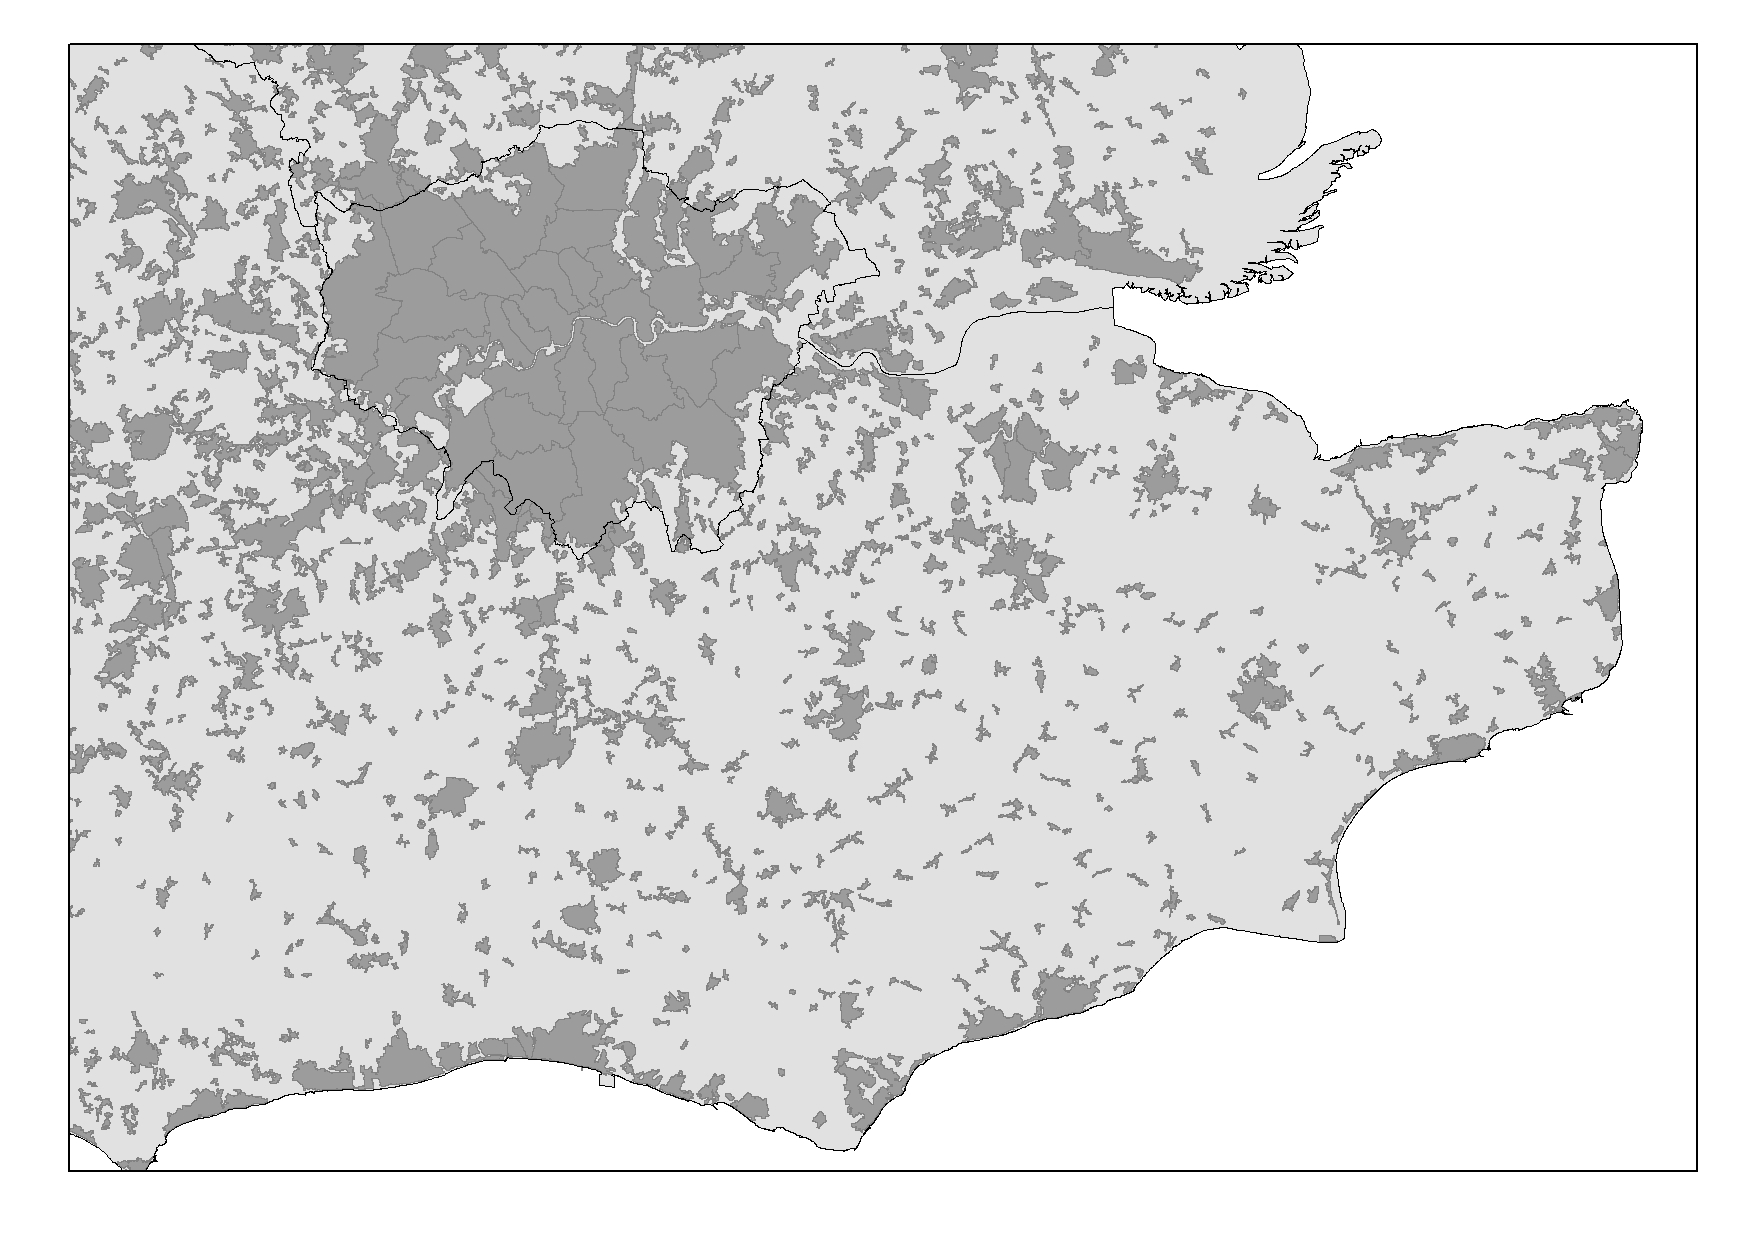
\includegraphics[width=0.8\linewidth]{Figure1} \caption{\label{figure1}Built-up areas in London and the South East of England}\label{fig:unnamed-chunk-11}
\end{figure}

In terms of our identification strategy, we follow the same approach as
we did for the US case. Table \ref{ols.uk} presents the OLS and GLM
estimation of equation \ref{eq4} while Table \ref{2sls.uk} presents the
2SLS estimation. Starting from Table \ref{ols.uk} we see a significant
and positive effect of the average download speed on the relative
position of a BUA in the urban hierarchy in England and Wales. This is
consistent with the previous results from the US and also with the
global model. Of course, the same endogeneity issues might be present
here too and we are addressing that below. In terms of control
variables, we include a measure of broadband tests per inhabitant in
order to control for potential differences in the take-up of this
service. In addition, we include a number of socio-economic variables
that we believe can affect the relative position of a city in the urban
hierarchy. Unemployment rate has a negative and significant effect as in
the US case. The same applies for the percentage of British population,
which indicates the importance of migration in urban growth. Population
density and the percentage of people working from home also negatively
affected the relative position of BUA during \(2011-2018\). Finally,
Table \ref{ols.uk} includes two interaction terms (columns \(2\) and
\(3\)) between download speed and population and population density. The
negative and significant sign for both interaction coefficients
indicates that the effect of download speed decreases as the size of the
BUA or its density increases. Contrary to the US case, this is
indicative of a larger digital connectivity effect for smaller BUA.

\begin{table}[!htbp] \centering 
  \caption{OLS and GLM estimations of equation (4) for the UK\label{ols.uk}} 
  \label{} 
\small 
\begin{tabular}{@{\extracolsep{1pt}}lcccc} 
\\[-1.8ex]\hline 
\hline \\[-1.8ex] 
 & \multicolumn{4}{c}{\textit{Dependent variable:}} \\ 
\cline{2-5} 
 & \multicolumn{4}{c}{Difference in ranks, 2013-18} \\ 
\\[-1.8ex] & (1) & (2) & (3) & (4)\\ 
\hline \\[-1.8ex] 
 download speed, 2011 (log) & 5.484$^{***}$ & 14.807$^{***}$ & 21.973$^{**}$ & 0.0004$^{***}$ \\ 
  & (2.029) & (5.348) & (8.791) & (0.0002) \\ 
  population, 2011 (log) & 5.720$^{***}$ & 5.808$^{***}$ & 23.875$^{***}$ & 0.0004$^{***}$ \\ 
  & (1.052) & (1.056) & (8.964) & (0.0001) \\ 
  broadband tests per capita, 2011 & $-$3.991 & $-$2.247 & $-$2.017 & $-$0.0003 \\ 
  & (10.382) & (10.556) & (10.471) & (0.001) \\ 
  \% of unemployment, 2011 & $-$142.544$^{***}$ & $-$140.509$^{***}$ & $-$142.753$^{***}$ & $-$0.011$^{***}$ \\ 
  & (53.532) & (53.629) & (53.493) & (0.004) \\ 
  \% of British population, 2011 & $-$34.756$^{**}$ & $-$42.859$^{**}$ & $-$39.608$^{**}$ & $-$0.003$^{**}$ \\ 
  & (16.009) & (16.687) & (16.466) & (0.001) \\ 
  population density, 2011 & 0.008 & 2.793$^{*}$ & 0.011 & 0.00000 \\ 
  & (0.150) & (1.571) & (0.150) & (0.00001) \\ 
  \% of people working from home, 2011 & $-$80.250$^{**}$ & $-$71.360$^{*}$ & $-$74.454$^{*}$ & $-$0.006$^{**}$ \\ 
  & (38.392) & (39.203) & (38.381) & (0.003) \\ 
  employment in service, 2011 (\%) & $-$61.945$^{**}$ & $-$62.921$^{**}$ & $-$64.734$^{**}$ & $-$0.005$^{**}$ \\ 
  & (28.073) & (28.066) & (28.098) & (0.002) \\ 
  download speed, 2011 (log) \\
                             x pop. density, 2011 &  & $-$0.338$^{*}$ &  &  \\ 
  &  & (0.183) &  &  \\ 
  download speed, 2011 (log) \\
                             x population, 2011 (log) &  &  & $-$2.175$^{**}$ &  \\ 
  &  &  & (1.080) &  \\ 
  Constant & $-$6.790 & $-$76.679 & $-$138.062$^{*}$ & 0.499$^{***}$ \\ 
  & (34.074) & (48.125) & (73.822) & (0.003) \\ 
 \hline \\[-1.8ex] 
Observations & 3,546 & 3,546 & 3,546 & 3,546 \\ 
Adjusted R$^{2}$ & 0.049 & 0.050 & 0.049 &  \\ 
Log Likelihood &  &  &  & 14,294.670 \\ 
Akaike Inf. Crit. &  &  &  & $-$28,571.330 \\ 
Residual Std. Error & 56.940 & 56.907 & 56.929 &  \\ 
\hline 
\hline \\[-1.8ex] 
\textit{Note:}  & \multicolumn{4}{r}{$^{*}$p$<$0.1; $^{**}$p$<$0.05; $^{***}$p$<$0.01} \\ 
 & \multicolumn{4}{r}{(1)-(3) is based on OLS, (4) on GLM} \\ 
 & \multicolumn{4}{r}{For the GLM the Normalized diff. in ranks is used} \\ 
 & \multicolumn{4}{r}{Robust std. errors in parenthesis} \\ 
\end{tabular} 
\end{table}

In regards to IV strategy, we use here the \emph{number of universities}
as the main instrument. Universities in England and Wales have been
established long time ago and therefore we do not expect them to affect
the change in the relative position of built-up areas in \(2011\). The
presence of universities and large student populations tend to be
correlated with the quality of internet infrastructure provision
{[}72{]}. The addition of the second instrument (absolute number of
broadband tests in 2011) in column \(2\) results to a Sargan test, the
null hypothesis of which cannot be rejected. Moreover, the estimations
reported in Table 11 do not suffer from weak instruments as the relevant
test is above the rule of thumb value of \(10\). The coefficients
derived from OLS (Table \ref{ols.uk}) and 2SLS (Table \ref{2sls.uk}) are
always positive and significant, something which advocates in favour of
the effect of broadband speed in enhancing agglomeration forces.
Interestingly, the magnitude of the 2SLS coefficient (column 1 in Table
\ref{2sls.uk}) is almost 8 times higher than the OLS coefficient (column
1 in Table \ref{ols.uk}). We attribute the OLS underestimation, which is
more or less consistent in all our estimations, to the difficulty in
directly observing active engagement with ICT. Our endogenous variable
captures the quality of the internet infrastructure as the experienced
internet speed. Similarly to the endogenous variables of the global and
the US model (internet and telephony take-up), what these variables do
not capture is what individuals actually do with ICT {[}73{]}. For
example, if we assume a bi-modal internet usage for either entertainment
or work purposes, one would expect that the latter would have a larger
effect on spatial structure than the former. We believe that our
endogenous variables capture mostly the former. Therefore, the IV
estimations, especially for UK case, reveal the local average treatment
effect {[}64{]} by capturing the effect of these users/households who
actively engage with ICT (e.g.~work on ICT-related sectors) and,
therefore, have a higher effect on spatial structure. A back of the
envelope calculation indicates that, everything else being equal, \(10\)
per cent increase in download speed for a BUA, would have increased its
position by \(4\) places.

\begin{table}[!htbp] \centering 
  \caption{2SLS estimation of equation (4) for the UK\label{2sls.uk}} 
  \label{} 
\small 
\begin{tabular}{@{\extracolsep{5pt}}lcc} 
\\[-1.8ex]\hline 
\hline \\[-1.8ex] 
 & \multicolumn{2}{c}{\textit{Dependent variable:}} \\ 
\cline{2-3} 
\\[-1.8ex] & \multicolumn{2}{c}{Difference in ranks, 2011-18} \\ 
\\[-1.8ex] & (1) & (2)\\ 
\hline \\[-1.8ex] 
 download speed, 2011 (log) & 43.058$^{***}$ & 47.226$^{***}$ \\ 
  & (11.727) & (6.298) \\ 
  population, 2011 (log) & $-$1.735 & $-$2.451$^{*}$ \\ 
  & (2.327) & (1.389) \\ 
  broadband tests per capita, 2011 & $-$6.658 & $-$5.763 \\ 
  & (12.159) & (12.263) \\ 
  \% of unemployment, 2011 & $-$93.185 & $-$89.366 \\ 
  & (60.397) & (59.332) \\ 
  \% of British population, 2011 & $-$36.963$^{**}$ & $-$38.269$^{**}$ \\ 
  & (17.921) & (17.631) \\ 
  population density, 2011 & $-$0.003 & $-$0.010 \\ 
  & (0.144) & (0.147) \\ 
  \% of people working from home, 2011 & $-$92.525$^{**}$ & $-$93.787$^{**}$ \\ 
  & (40.412) & (40.729) \\ 
  employment in service, 2011 (\%) & $-$47.395$^{*}$ & $-$48.132$^{*}$ \\ 
  & (28.089) & (28.448) \\ 
  Constant & $-$260.358$^{***}$ & $-$286.509$^{***}$ \\ 
  & (81.193) & (51.613) \\ 
 \hline \\[-1.8ex] 
Weak instruments & 6.98 & 42.03 \\ 
Wu-Hausman & 8.08 & 40.8 \\ 
P-value & 0 & 0 \\ 
Sargan &  & 0.02 \\ 
P-value &  & 0.9 \\ 
Observations & 3,032 & 3,032 \\ 
Adjusted R$^{2}$ & $-$0.069 & $-$0.096 \\ 
Residual Std. Error & 57.001 & 57.721 \\ 
\hline 
\hline \\[-1.8ex] 
\textit{Note:}  & \multicolumn{2}{r}{$^{*}$p$<$0.1; $^{**}$p$<$0.05; $^{***}$p$<$0.01} \\ 
 & \multicolumn{2}{r}{Robust std. errors in parenthesis} \\ 
 & \multicolumn{2}{r}{IVs: (1) N.r of universities} \\ 
 & \multicolumn{2}{r}{IVs: (2) N. of universities, N. of broadband tests, 2011} \\ 
 & \multicolumn{2}{r}{First stage regressions can be found in S3} \\ 
\end{tabular} 
\end{table}

In total, the results of the UK case study are in accordance with the
previous results of the global, multi-country analysis and of the US
urban system. Interestingly, the positive effect of internet is still
apparent when the analysis adopts a morphological definition of cities
and when the emphasis is not on internet penetration, but instead on the
quality of internet infrastructure as reflected in download broadband
speed. What is also interesting for the UK case study is that this
effect appears to be higher for small and less dense BUA.

\hypertarget{sec6}{%
\section{Discussion and conclusions}\label{sec6}}

This paper reports empirical findings on a question at the heart of
urban economics and economic geography: has the proliferation of
information and communication technologies offset the benefits of
agglomeration economies and resulted in more dispersed spatial
population structures, or has it further reinforced such urban
externalities and led to more concentrated spatial structures? Previous
studies have led to contradictory results regarding whether ICT adoption
and urban agglomeration externalities are complementary or
substitutable. As Leamer and Storper {[}33{]} stress, the internet can
affect both centripetal and centrifugal forces. The present study
revisits Ioannides et al.~{[}18{]} with a completely open mind in view
of the availability of several years of additional data on internet
penetration across the world. It examines the robustness of the findings
of Tranos and Ioannides {[}19{]} by employing alternative data sets. In
general, quite a few earlier studies have either been based on
assumptions about technological capabilities that might no longer hold
today, or use data that do not fully capture the widespread adoption and
maturity of communication technologies that has taken place since the
data coverage of those earlier studies.

We report estimation results using international country-level data on
urban agglomerations with more than \(300,000\) inhabitants from the UN
Urban Settlements data and test the effect of ICT adoption on the Pareto
exponents for national city size distributions, as measures of
dispersion for heavy-tailed data. We report results which are robust to
endogeneity concerns. Then, in order to examine such effects for cities
that are smaller than those included in our international data, we focus
on the US and the UK urban systems. Specifically, we test the effect of
internet usage and internet speed on the changes over time in rankings
of Micropolitan and Metropolitan Areas in the US, and of Built Up Areas
in the UK. The results favor a complementary relation between the
internet and agglomeration externalities. While the cross-country
estimates indicate that increase adoption rates of such technologies has
resulted in less dispersed urban spatial structures, the two case
studies reveal that internet adoption and internet speed improved the
relative population rank of a city within its urban system.
Interestingly, the latter results indicate that such effects might be
even stronger for smaller and less dense urban areas at least in the UK.
On the contrary, our estimates regarding the effect of fixed telephony
advocate towards the reverse effect: that is fixed telephony acting
against of agglomeration forces.

While our results are in agreement with Ioannides et al.~{[}18{]}
regarding fixed telephony, they contradict Tranos and Ioannides {[}19{]}
The latter cannot of course be ignored. We believe strongly that the
differences lie in the different definitions of urban areas. To this
date, and in spite of numerous efforts by teams worldwide, there has not
been a universally accepted definition, which could moreover be
implemented consistently by governments worldwide. The increasingly
popular reliance on high-resolution, pioneered by Rozenfeld et
al.~{[}74{]}, and satellite-based lights data, most recently used by
Duben and Krause {[}75{]}, for measuring city sizes, are very exciting
developments, but they have not yet been accompanied by complementary
information on ICT adoption at a comparably granular level. A promising
new development is the EU's Global Human Settlements Initiative and the
associated spatial urban data sets; see Pesaresi et al.~{[}76{]}.
Barring the availability of such data, scholars must be careful in
drawing conclusions. Arguably, the measurement of the impact of ICT at
the level of agglomerations, on one hand, and on changes in rankings, on
the other, reported by this paper constitute a contribution to the
literature.

We believe that our results, apart from their theoretical value, have
the capacity to inform urban policy. The ability of the internet and
digital communications to further enhance agglomeration economies can be
used as a tool to support urban growth. In addition, the indication that
such effects might be stronger for smaller and less dense urban areas,
at least in England and Wales, might be helpful to further orient
digital strategies towards such locations. Of course, improvements in
internet speed is not a trivial policy instrument as it involves
numerous complexities. Apart from infrastructure installation costs and
engineering challenges, governance issues regarding the ownership of
such digital networks as well as the provision of state subsidies create
obstacles for the inclusion of such strategies in the urban growth
agenda. To further inform such policies, more research at granular
scales is needed in order to shed lights on the micro-mechanisms behind
such urban processes.

\hypertarget{references}{%
\section*{References}\label{references}}
\addcontentsline{toc}{section}{References}

\hypertarget{refs}{}
\leavevmode\hypertarget{ref-toffler_third_1980}{}%
1. Toffler A. Third way. New York: William Morrow; 1980.

\leavevmode\hypertarget{ref-ohmae_borderless_1995}{}%
2. Ohmae K. The Borderless World: Power and Strategy in an
Interdependent Economy. New York: Harper Business; 1995.

\leavevmode\hypertarget{ref-gilder_notitle_1995}{}%
3. Gilder G. Forbes ASAP. 1995; 56.

\leavevmode\hypertarget{ref-peter_f_drucker_capitalism_1998}{}%
4. Drucker PF. From Capitalism to Knowledge Society. In: Neef D, editor.
The knowledge economy. Woburn, MA: Butterworth-Heinemann; 1998. pp.
15--34.

\leavevmode\hypertarget{ref-obrien_global_1992}{}%
5. O'Brien R. Global Financial Integration: The End of Geography.
London: Pinter; 1992.

\leavevmode\hypertarget{ref-frances_cairncross_death_2001}{}%
6. Cairncross F. The death of distance 2.0. London: Texere Publishing
Limited; 2001.

\leavevmode\hypertarget{ref-friedman_world_2005}{}%
7. Friedman TL. The world is flat. New York: Farrar, Straus; Giroux;
2005.

\leavevmode\hypertarget{ref-kende_digital_2003}{}%
8. Kende M. The digital handshake: Connecting Internet backbones.
CommLaw Conspectus. 2003;11: 45.

\leavevmode\hypertarget{ref-united_nations_world_2014}{}%
9. Nations U. World Urbanization Prospects: The 2014 Revision.
Department of Economic; Social Affairs, Population Division, UN; 2014.

\leavevmode\hypertarget{ref-panahi_towards_2013}{}%
10. Panahi S, Watson J, Partridge H. Towards tacit knowledge sharing
over social web tools. Journal of Knowledge Management. 2013;17:
379--397.

\leavevmode\hypertarget{ref-storper_buzz_2004}{}%
11. Storper M, Venables AJ. Buzz: Face-to-face contact and the urban
economy. Journal of economic geography. 2004;4: 351--370.

\leavevmode\hypertarget{ref-tranos2020social}{}%
12. Tranos E. Social network sites and knowledge transfer: An urban
perspective. Journal of Planning Literature. SAGE Publications Sage CA:
Los Angeles, CA; 2020; 0885412220921526.

\leavevmode\hypertarget{ref-rosenthal_evidence_2004}{}%
13. Rosenthal SS, Strange WC. Evidence on the nature and sources of
agglomeration economies. Handbook of regional and urban economics.
2004;4: 2119--2171.

\leavevmode\hypertarget{ref-mccann_globalization_2008}{}%
14. McCann P. Globalization and economic geography: The world is curved,
not flat. Cambridge Journal of Regions, Economy and Society. 2008;1:
351--370.

\leavevmode\hypertarget{ref-duranton_micro-foundations_2004}{}%
15. Duranton G, Puga D. Micro-foundations of urban agglomeration
economies. Handbook of regional and urban economics. 2004;4: 2063--2117.

\leavevmode\hypertarget{ref-van_dijck_you_2013}{}%
16. Van Dijck J. ``You have one identity'': Performing the self on
Facebook and LinkedIn. Media, Culture \& Society. 2013;35: 199--215.

\leavevmode\hypertarget{ref-gee2019more}{}%
17. Gee LK. The more you know: Information effects on job application
rates in a large field experiment. Management Science. INFORMS; 2019;65:
2077--2094.

\leavevmode\hypertarget{ref-ioannides2008effect}{}%
18. Ioannides YM, Overman HG, Rossi-Hansberg E, Schmidheiny K. The
effect of information and communication technologies on urban structure.
Economic Policy. Oxford University Press; 2008;23: 202--242.

\leavevmode\hypertarget{ref-tranos2020ict}{}%
19. Tranos E, Ioannides YM. ICT and cities revisited. Telematics and
Informatics. Elsevier; 2020; 101439.

\leavevmode\hypertarget{ref-jess_gaspar_information_1998}{}%
20. Gaspar J, Glaeser EL. Information Technology and the Future of
Cities. Journal of Urban Economics. 1998;43: 136--156.

\leavevmode\hypertarget{ref-hildrum_sharing_2009}{}%
21. Hildrum JM. Sharing Tacit Knowledge Online: A Case Study of
e-Learning in Cisco's Network of System Integrator Partner Firms.
Industry and Innovation. 2009;16: 197--218.

\leavevmode\hypertarget{ref-kolko_death_2000}{}%
22. Kolko J. The death of cities? The death of distance? Evidence from
the geography of commercial Internet usage. In: Vogelsang I, Compaine
BM, editors. The internet upheaval: Raising questions, seeking answers
in communications policy. Cambridge, MA; London, UK: The MIT Press;
2000. pp. 73--98.

\leavevmode\hypertarget{ref-todd_sinai_geography_2004}{}%
23. Sinai T, Waldfogel J. Geography and the Internet: Is the Internet a
substitute or a complement for cities? Journal of Urban Economics.
2004;56: 1--24.

\leavevmode\hypertarget{ref-chris_forman_how_2005}{}%
24. Forman C, Goldfarb A, Greenstein S. How did location affect adoption
of the commercial Internet? Global village vs. Urban leadership. Journal
of Urban Economics. 2005;58: 389--420.

\leavevmode\hypertarget{ref-jungyul_sohn_information_2003}{}%
25. Sohn J, Kim TJ, Hewings GJD. Information technology and urban
spatial structure: A comparative analysis of the Chicago and Seoul
regions. Annals of Regional Science. 2003;37: 447--462.

\leavevmode\hypertarget{ref-pons-novell_cities_2006}{}%
26. Pons-Novell J, Viladecans-Marsal E. Cities and the Internet: The end
of distance? Journal of Urban Technology. 2006;13: 109--132.

\leavevmode\hypertarget{ref-craig_does_2016}{}%
27. Craig SG, Hoang EC, Kohlhase JE. Does closeness in virtual space
complement urban space? Socio-Economic Planning Sciences. 2016;

\leavevmode\hypertarget{ref-mark_d_partridge_employment_2008}{}%
28. Partridge MD, Rickman DS, Ali K, Olfert MR. Employment Growth in the
American Urban Hierarchy: Long Live Distance. The BE Journal of
Macroeconomics. 2008;8: Article 10.

\leavevmode\hypertarget{ref-kim_broadband_2016}{}%
29. Kim Y, Orazem PF. Broadband Internet and New Firm Location Decisions
in Rural Areas. American Journal of Agricultural Economics. 2016;99:
285--302.

\leavevmode\hypertarget{ref-bekkerman_high-speed_2013}{}%
30. Bekkerman A, Gilpin G. High-speed Internet growth and the demand for
locally accessible information content. Journal of Urban Economics.
2013;77: 1--10.

\leavevmode\hypertarget{ref-anenberg_information_2015}{}%
31. Anenberg E, Kung E. Information technology and product variety in
the city: The case of food trucks. Journal of Urban Economics. 2015;90:
60--78.

\leavevmode\hypertarget{ref-rietveld_transport_2004}{}%
32. Rietveld P, Vickerman RW. Transport in regional science: The ``death
of distance'' is premature. Papers in Regional Science. 2004;83:
229--248.

\leavevmode\hypertarget{ref-edward_e_leamer_economic_2001}{}%
33. Leamer EE, Storper M. The Economic Geography of the Internet Age.
Journal of International Business Studies. 2001;32: 641--65.

\leavevmode\hypertarget{ref-pew_internet_pew_2016}{}%
34. Internet P. Pew Internet \& American Life Project. Pew Internet;
2016.

\leavevmode\hypertarget{ref-internet_live_stats_internet_2017}{}%
35. Stats IL. Internet Users. 2017.

\leavevmode\hypertarget{ref-fb}{}%
36. Facebook. Facebook company information. 2021. Available:
\url{http://newsroom.fb.com/company-info/}

\leavevmode\hypertarget{ref-dingel2020many}{}%
37. Dingel JI, Neiman B. How many jobs can be done at home? National
Bureau of Economic Research; 2020.
doi:\href{https://doi.org/DOI\%2010.3386/w26948}{DOI 10.3386/w26948}

\leavevmode\hypertarget{ref-black_urban_2003}{}%
38. Black D, Henderson V. Urban evolution in the USA. Journal of
economic geography. 2003;3: 343--372.

\leavevmode\hypertarget{ref-frenken_theoretical_2007}{}%
39. Frenken K, Boschma RA. A theoretical framework for evolutionary
economic geography: Industrial dynamics and urban growth as a branching
process. Journal of economic geography. 2007;7: 635--649.

\leavevmode\hypertarget{ref-giesen_zipfs_2011}{}%
40. Giesen K, Südekum J. Zipf's law for cities in the regions and the
country. Journal of economic geography. 2011;11: 667--686.

\leavevmode\hypertarget{ref-rauch_cities_2013}{}%
41. Rauch F. Cities as spatial clusters. Journal of economic geography.
2013; lbt034.

\leavevmode\hypertarget{ref-ioannides_zipfs_2003}{}%
42. Ioannides YM, Overman HG. Zipf's law for cities: An empirical
examination. Regional science and urban economics. 2003;33: 127--137.

\leavevmode\hypertarget{ref-ioannides_walled_2017}{}%
43. Ioannides YM, Zhang J. Walled cities in late imperial China. Journal
of Urban Economics. 2017;97: 71--88.

\leavevmode\hypertarget{ref-nitsch_zipf_2005}{}%
44. Nitsch V. Zipf zipped. Journal of Urban Economics. 2005;57: 86--100.

\leavevmode\hypertarget{ref-gabaix_evolution_2004}{}%
45. Gabaix X, Ioannides YM. The evolution of city size distributions.
Handbook of regional and urban economics. 2004;4: 2341--2378.

\leavevmode\hypertarget{ref-gabaix_rank_2011}{}%
46. Gabaix X, Ibragimov R. Rank− 1/2: A simple way to improve the OLS
estimation of tail exponents. Journal of Business \& Economic
Statistics. 2011;29: 24--39.

\leavevmode\hypertarget{ref-ioannides2013neighborhoods}{}%
47. Ioannides Y. From neighborhoods to nations: The economics of social
interactions. Princeton University Press; 2013.

\leavevmode\hypertarget{ref-citypop}{}%
48. Brinkhoff T. City population. 2021. Available:
\url{http://www.citypopulation.de}

\leavevmode\hypertarget{ref-soo_zipfs_2005}{}%
49. Soo KT. Zipf's Law for cities: A cross-country investigation.
Regional science and urban economics. 2005;35: 239--263.
doi:\href{https://doi.org/http://dx.doi.org/10.1016/j.regsciurbeco.2004.04.004}{http://dx.doi.org/10.1016/j.regsciurbeco.2004.04.004}

\leavevmode\hypertarget{ref-cohen_urban_2004}{}%
50. Cohen B. Urban growth in developing countries: A review of current
trends and a caution regarding existing forecasts. World development.
2004;32: 23--51.

\leavevmode\hypertarget{ref-montgomery_urban_2008}{}%
51. Montgomery MR. The urban transformation of the developing world.
science. 2008;319: 761--764.

\leavevmode\hypertarget{ref-chen_absolute_2007}{}%
52. Chen S, Ravallion M. Absolute poverty measures for the developing
world, 1981--2004. Proceedings of the National Academy of Sciences.
2007;104: 16757--16762.

\leavevmode\hypertarget{ref-decker_global_2007}{}%
53. Decker EH, Kerkhoff AJ, Moses ME. Global patterns of city size
distributions and their fundamental drivers. PLoS One. 2007;2: e934.

\leavevmode\hypertarget{ref-donner_research_2008}{}%
54. Donner J. Research approaches to mobile use in the developing world:
A review of the literature. The information society. 2008;24: 140--159.

\leavevmode\hypertarget{ref-hamilton_are_2003}{}%
55. Hamilton J. Are main lines and mobile phones substitutes or
complements? Evidence from Africa. Telecommunications Policy. 2003;27:
109--133.

\leavevmode\hypertarget{ref-batty_rank_2006}{}%
56. Batty M. Rank clocks. Nature. 2006;444: 592--596.

\leavevmode\hypertarget{ref-havlin_distance_1995}{}%
57. Havlin S. The distance between Zipf plots. Physica A: Statistical
Mechanics and its Applications. 1995;216: 148--150.

\leavevmode\hypertarget{ref-chetty2018impacts}{}%
58. Chetty R, Hendren N. The impacts of neighborhoods on
intergenerational mobility i: Childhood exposure effects. The Quarterly
Journal of Economics. Oxford University Press; 2018;133: 1107--1162.

\leavevmode\hypertarget{ref-dettling2017}{}%
59. Dettling LJ. Broadband in the labor market: The impact of
residential high-speed internet on married women's labor force
participation. ILR Review. 2017;70: 451--482.
doi:\href{https://doi.org/10.1177/0019793916644721}{10.1177/0019793916644721}

\leavevmode\hypertarget{ref-arntz2019working}{}%
60. Arntz M, Sarra BY, Berlingieri F. Working from home: Heterogeneous
effects on hours worked and wages. ZEW-Centre for European Economic
Research Discussion Paper. 2019;

\leavevmode\hypertarget{ref-watson2018digitalisation}{}%
61. Watson T, Corliss M, Le M, others. Digitalisation and women's
workforce participation in the indo-pacific. Australian Journal of
Labour Economics. Centre for Labour Market Research; 2018;21: 45.

\leavevmode\hypertarget{ref-Lechman2020}{}%
62. Lechman E, Popowska M. Enhancing women's engagement in economic
activities through information and communication technology deployment:
Evidence from central--eastern european countries. Gender, Technology
and Development. Routledge; 2020;24: 314--340.
doi:\href{https://doi.org/10.1080/09718524.2020.1824568}{10.1080/09718524.2020.1824568}

\leavevmode\hypertarget{ref-Valberg2020}{}%
63. Valberg S. ICT, gender, and the labor market: A cross-country
analysis. In: Maiti D, Castellacci F, Melchior A, editors.
Digitalisation and development: Issues for india and beyond. Singapore:
Springer Singapore; 2020. pp. 375--405.
doi:\href{https://doi.org/10.1007/978-981-13-9996-1_15}{10.1007/978-981-13-9996-1\_15}

\leavevmode\hypertarget{ref-angrist1995identification}{}%
64. Angrist JD, Imbens GW. Identification and estimation of local
average treatment effects. National Bureau of Economic Research; 1995.

\leavevmode\hypertarget{ref-calabrese2011interplay}{}%
65. Calabrese F, Smoreda Z, Blondel VD, Ratti C. Interplay between
telecommunications and face-to-face interactions: A study using mobile
phone data. PloS one. Public Library of Science; 2011;6: e20814.

\leavevmode\hypertarget{ref-buchel2020cities}{}%
66. Büchel K, Ehrlich MV. Cities and the structure of social
interactions: Evidence from mobile phone data. Journal of Urban
Economics. Elsevier; 2020;119: 103276.

\leavevmode\hypertarget{ref-file_computer_2014}{}%
67. File T, Ryan C. Computer and Internet use in the United States:
2013. American Community Survey Reports. 2014;

\leavevmode\hypertarget{ref-riddlesden_broadband_2014}{}%
68. Riddlesden D, Singleton AD. Broadband speed equity: A new digital
divide? Applied Geography. 2014;52: 25--33.

\leavevmode\hypertarget{ref-ons2013}{}%
69. ONS. 2011 Built-up Areas - Methodology and Guidance. Office for
National Statistics; 2013 pp. 1--15.

\leavevmode\hypertarget{ref-johnston_changing_2014}{}%
70. Johnston R, Poulsen M, Forrest J. The changing ethnic composition of
urban neighbourhoods in England and Wales, 2001-2011: Creating nations
of strangers? Geography. 2014;99: 67.

\leavevmode\hypertarget{ref-johnston2016ethnic}{}%
71. Johnston R, Poulsen M, Forrest J. Ethnic residential patterns in
urban england and wales, 2001--2011: A system-wide analysis. Tijdschrift
voor economische en sociale geografie. Wiley Online Library; 2016;107:
1--15.

\leavevmode\hypertarget{ref-GRUBESIC201950}{}%
72. Grubesic TH, Helderop E, Alizadeh T. Closing information
asymmetries: A scale agnostic approach for exploring equity implications
of broadband provision. Telecommunications Policy. 2019;43: 50--66.
doi:\href{https://doi.org/https://doi.org/10.1016/j.telpol.2018.04.002}{https://doi.org/10.1016/j.telpol.2018.04.002}

\leavevmode\hypertarget{ref-tranos2020digital}{}%
73. Tranos E, Kitsos T, Ortega-Argilés R. Digital economy in the uk:
Regional productivity effects of early adoption. Regional Studies.
Routledge; 2020; 1--15.

\leavevmode\hypertarget{ref-rozenfeld2011area}{}%
74. Rozenfeld HD, Rybski D, Gabaix X, Makse HA. The area and population
of cities: New insights from a different perspective on cities. American
Economic Review. 2011;101: 2205--25.

\leavevmode\hypertarget{ref-duben2019population}{}%
75. Duben C, Krause M, others. Population, light, and the size
distribution of cities. 2019.

\leavevmode\hypertarget{ref-pesaresi2019ghs}{}%
76. Pesaresi M, Florczyk A, Schiavina M, Melchiorri M, Maffenini L. GHS
settlement grid, updated and refined regio model 2014 in application to
ghs-built r2018a and ghs-pop r2019a, multitemporal (1975-1990-2000-2015)
r2019a. European Commission, Joint Research Centre (JRC). 2019;

\nolinenumbers


\end{document}

